% Appendix B

\chapter{Appendix for Chapter \ref{Chapter4}}
\label{AppendixB}
\lhead{Appendix \ref{AppendixB}. \emph{Appendix for Chapter \ref{Chapter4}}}

We provide, in this Appendix, additional material that complements the exposition of the PESMOC approach introduced in Chapter \ref{Chapter4}. Concretely, we show the exact computations done by the expectation propagation algorithm to approximate the intractable factors of the conditional predictive distribution involved in the PESMOC acquisition function approximation. We also include a sensitivity analysis of the number of Monte Carlo iterations of the Slice sampling algorithm. Additionaly, we include another sensitivity analysis of the sampled Pareto sets and an analysis of the infeasible solutions in benchmark experiments.

\section{The Gaussian Approximation to the Conditional Predictive Distribution}

Recall from the main manuscript that, in this work, we wish to approximate the Conditional Predictive Distribution of the set defined by the points $\mathcal{X} = \{\{\boldsymbol{x}_n\}_{n=1}^{N} \cup \mathcal{X}^* \cup \{\boldsymbol{x}\}\}$. This set is, the union between the $\mathcal{N}$ observation points in the input space $\{\boldsymbol{x}_n\}_{n=1}^{N}$, the $\mathcal{M}$ Pareto Set points $\mathcal{X}^*$ and the candidate point $\{\boldsymbol{x}\}$ to be evaluated. The Gaussian Approximation will then be a multivariate Gaussian Distribution over $\mathcal{N}$+$\mathcal{M}$+1 variables. The Conditional Predictive Distribution is given by the following expression
\begin{align}
p(\textbf{y}|\mathcal{D}, \textbf{x}, \mathcal{X}^{\star}) & \propto 
        \int p(\textbf{y}|\textbf{x},\textbf{f},\textbf{c}) 
        p(\mathcal{X}^{\star}|\textbf{f},\textbf{c}) p(\textbf{f}|\mathcal{D}) p(\textbf{c}|\mathcal{D})
 d\textbf{f} d\textbf{c}
\end{align}\,,
where $p(\textbf{y}|\textbf{x},\textbf{f},\textbf{c}) = \prod_{k=1}^{K}\delta(y_k - f_k(\textbf{x})) 
\prod_{j=1}^{J}\delta (y_{K+j} - c_j(\textbf{x}))$ and $p(\mathcal{X}^{\star}|\textbf{f},\textbf{c})$ is given by
\begin{align}
\hspace{-.2cm}
p(\mathcal{X}^{\star}|\textbf{f},\textbf{c}) & \propto 
        \prod_{\textbf{x}^\star\in \mathcal{X}^\star} 
        \left(
        \Bigg[\prod_{j=1}^{J}\Phi_j(\textbf{x}^{\star})\Bigg]
        \left[ 
        \prod_{\textbf{x}'\in \mathcal{X}} 
        \Omega(\textbf{x}',\textbf{x}^{\star})
        \right] 
        \right)
        \,,
        \label{eq:x_star}
\end{align}
where $\Phi_j(\mathbf{x}^\star) = \Theta(c_j(\mathbf{x}^\star))$ with $\Theta(\cdot)$ the Heaviside step function,
and $\Omega(\textbf{x}',\textbf{x}^{\star})$ is defined as:

\begin{align}
\Omega(\textbf{x}',\textbf{x}^{\star}) & = \left[\prod_{j=1}^{J}\Theta(c_j(\mathbf{x}'))\right] 
        \psi(\textbf{x}',\textbf{x}^{\star}) + \left[1 - \prod_{j=1}^{J}\Theta(c_j(\textbf{x}')) \right] \cdot 1
\,,
        \label{eq:omega}
\end{align}
where $\psi(\textbf{x}',\textbf{x}^{\star})$ is defined as
\begin{align}
\psi(\textbf{x}',\textbf{x}^{\star}) & = 1 - \prod_{k=1}^K \Theta (f_k(\textbf{x}^{\star})-f_k(\textbf{x}'))
\,.  \label{eq:psi}
\end{align}
The last two probability densities, $p(\textbf{f}|\mathcal{D})$ and $p(\textbf{c}|\mathcal{D})$ , involved in the Conditional Predictive Distribution are potentially infinite-dimensional Gaussians given by the Gaussian Process predictive distributions for the objectives $\textbf{f}$ and constraints $\textbf{c}$ values. As these distributions are Gaussian, they do not need to be approximated.

In order to find a Gaussian Approximation to Eq.(4) it is necessary to perform several steps. First of all, we separate the factors that depend and not depend on \textbf{x} so that they will be approximated separately. By doing this, the factors that depend on $\boldsymbol{x}$ are refined only once by EP and the other factors are refined iteratively by EP until they change no more.

The factors that depend on \textbf{x} are the Dirac Delta functions that can be replaced by Gaussians with the corresponding noise variance in the noise case and no variance in the noiseless case. As they are Gaussian Distributions, there is nothing to approximate.

The other factors are the ones that do not depend on \textbf{x}. We define the sampled Pareto Set as $\mathcal{X}^{*} = \{\boldsymbol{x}^{*}_{1},...,\boldsymbol{x}^{*}_{M}\}$ of size $\mathcal{M}$ and the set of $\mathcal{N}$ observations in the input space as $\hat{\mathcal{X}} = \{\boldsymbol{x}_1,...,\boldsymbol{x}_N\}$ with the corresponding observations of the k-th objective $\boldsymbol{y}_k$ and of the c-th constraint $\boldsymbol{y}_j$. Then, the values of the posterior distributions of the GPs of the objectives and the constraints at that points are defined by $\boldsymbol{f}_k = ( f_k(\boldsymbol{x}^{*}_1), ... , f_k(\boldsymbol{x}^{*}_M), f_k(\boldsymbol{x}_1),  f_k(\boldsymbol{x}_N))^T$ and $\boldsymbol{c}_j = ( c_j(\boldsymbol{x}^{*}_1), ... , c_j(\boldsymbol{x}^{*}_M), c_j(\boldsymbol{x}_1), c_j(\boldsymbol{x}_N))^T$. If we define $\boldsymbol{f} = \{\boldsymbol{f}_1,...,\boldsymbol{f}_K\}$ and $\boldsymbol{c} = \{\boldsymbol{c}_1,...,\boldsymbol{c}_J\}$, let $q(\boldsymbol{f},\boldsymbol{c})$ be the distribution that we want to approximate, $p(\mathcal{X}^{\star}|\textbf{f},\textbf{c}) p(\textbf{f}|\mathcal{D}) p(\textbf{c}|\mathcal{D})$, with the factors that do not depend on \textbf{x}, that is:

\begin{align}
q(\boldsymbol{f},\boldsymbol{c}) = \prod_{\textbf{x}^\star\in \mathcal{X}^\star} 
        \left(
        \Bigg[\prod_{j=1}^{J}\Phi_j(\textbf{x}^{\star})\Bigg]
        \left[ 
        \prod_{\textbf{x}'\in \mathcal{X}} 
        \Omega(\textbf{x}',\textbf{x}^{\star})
        \right] 
        \right)
p(\textbf{f}|\mathcal{D}) p(\textbf{c}|\mathcal{D})
 d\textbf{f} d\textbf{c}\,.
\end{align}
Because Eq.(10) is not tractable, we approximate the normalized version of $q(\boldsymbol{f},\boldsymbol{c})$ with a product of Gaussians, the Gaussian Approximation to the Conditional Predictive Distribution. Eq.(10) can be expressed as this normalized product:
\begin{align}
q(\boldsymbol{f},\boldsymbol{c}) & = \frac{1}{Z_q} \bigg[\prod_{k=1}^{K}\mathcal{N}\big(\boldsymbol{f}_k\ |\  \boldsymbol{m}_{pred}^{\boldsymbol{f}_k}, \boldsymbol{V}_{pred}^{\boldsymbol{f}_k}\big)\bigg] \bigg[\prod_{j=1}^{J}\mathcal{N}\big(\boldsymbol{c}_j\ |\  \boldsymbol{m}_{pred}^{\boldsymbol{c}_j}, \boldsymbol{V}_{pred}^{\boldsymbol{c}_j}\big)\bigg] \times \nonumber
\\
        & \quad \prod_{\textbf{x}^\star\in \mathcal{X}^\star} 
        \left(
        \Bigg[\prod_{j=1}^{J}\Phi_j(\textbf{x}^{\star})\Bigg]
        \left[ 
        \prod_{\textbf{x}'\in \mathcal{X}} 
        \Omega(\textbf{x}',\textbf{x}^{\star})
        \right] 
        \right)\,,
\end{align}
where $\boldsymbol{m}_{pred}^{\boldsymbol{f}_k}$ and $\boldsymbol{V}_{pred}^{\boldsymbol{f}_k}$ are the mean and covariance matrix of the posterior distributions of $\boldsymbol{f}_k$ given the data in $\mathcal{D}$ and $\boldsymbol{m}_{pred}^{\boldsymbol{c}_j}$ and $\boldsymbol{V}_{pred}^{\boldsymbol{c}_j}$ are the mean and covariance matrix of the posterior distribution of $\boldsymbol{c}_j$ given the data in $\mathcal{D}$. These means and variances are computed according to the equations 2.22-2.24 provided by Rasmussen \citep{rasmussen2003gaussian}:
\begin{align}
    &
    \boldsymbol{m}_{pred}^{\boldsymbol{f}_{k}} = \boldsymbol{K}_{*}^{k}\big(\boldsymbol{K}^{f} + v_{f}^{2}        \mathds{I}\big)^{-1}\boldsymbol{y}^k\,, \nonumber \\
    & 
    \boldsymbol{V}_{pred}^{\boldsymbol{f}_{k}} = \boldsymbol{K}_{*,*}^{k} - \boldsymbol{K}_{*}^{k}\big(\boldsymbol{K}^{k} + v_{f}^{2}        \mathds{I}\big)^{-1}\big[\boldsymbol{K}_{*}^{k}\big]\,,
\end{align}
where $\boldsymbol{K}_{*}^{k}$ is an $(N + 1) \times N$ matrix with the prior cross-covariances between elements of $\boldsymbol{f}_k$ and $f_{k,1},...,f_{k,n}$ and $\boldsymbol{K}_{*,*}^{k}$ is an $(N + 1) \times (N + 1)$ matrix with the prior covariances between the elements of $\boldsymbol{f}_k$ and $v_k$ is the standard deviation of the additive Gaussian noise in the evaluations of $\boldsymbol{f}_k$. Following the same reasoning, we have that:
\begin{align}
    &
    \boldsymbol{m}_{pred}^{\boldsymbol{c}_{j}} = \boldsymbol{K}_{*}^{j}\big(\boldsymbol{K}^{j} + v_{j}^{2}        \mathds{I}\big)^{-1}\boldsymbol{y}^j\,, \nonumber \\
    & 
    \boldsymbol{V}_{pred}^{\boldsymbol{c}_{j}} = \boldsymbol{K}_{*,*}^{j} - \boldsymbol{K}_{*}^{j}\big(\boldsymbol{K}^{j} + v_{j}^{2}        \mathds{I}\big)^{-1}\big[\boldsymbol{K}_{*}^{j}\big]\,,
\end{align}
where $\boldsymbol{K}_{*}^{j}$ is an $(N + 1) \times N$ matrix with the prior cross-covariances between elements of $\boldsymbol{c}_j$ and $c_{j,1},...,c_{j,n}$ and $\boldsymbol{K}_{*,*}^{j}$ is an $(N + 1) \times (N + 1)$ matrix with the prior covariances between the elements of $\boldsymbol{c}_j$ and $v_j$ is the standard deviation of the additive Gaussian noise in the evaluations of $\boldsymbol{c}_j$.

The other non-Gaussian factors presented in Eq.(11), $\Phi_j(\textbf{x}^{\star})$ and  $\Omega(\textbf{x}',\textbf{x}^{\star})$, are the problematic ones, as they are not Gaussian Distributions. Hence they will be approximated by Gaussians with EP, as will be described in the next sections.

\section{Using Expectation Propagation to Approximate the Conditional Predictive Distribution}

This section explains how the EP algorithm approximate the previous product of factors, giving a product of Gausssian Distributions which we call the Gaussian Approximation to the Conditional Predictive Distribution, shown in the previous section. As it is a product where different factors are involved, we have to divide the problem in the approximation of the different factors for Gaussian Distributions. These are the $\Phi_j(\boldsymbol{x}^*$ factors and the $\Omega(\textbf{x}',\textbf{x}^{\star})$ factors, which will be approximated by one-dimensional and two-dimensional Gaussian Distributions respectively.

The factors $\Phi(\boldsymbol{x}^*)$ that represent if a Pareto Set point $\boldsymbol{x}^*$ is feasible evaluated in a certain constraint $c_j(\boldsymbol{x}^*)$, are approximated by a one-dimensional un-normalized Gaussian distribution $\tilde{\Phi}(\boldsymbol{x}^*)$. This distribution is expressed in exponential family form in the next equation:
\begin{align}
    \Phi(\boldsymbol{x}^*) \approx \tilde{\Phi}(\boldsymbol{x}^*) \propto \exp\bigg\{ - \frac{c_j(\boldsymbol{x}^{*})^{2}\hat{v}_{j}^{\boldsymbol{x}^{*}}}{2} + c_j(\boldsymbol{x}^*)\hat{m}_{j}^{\boldsymbol{x}^*}\bigg\}\,,
\end{align}
where $\hat{v}_{j}^{\boldsymbol{x}^{*}}$ and $\hat{m}_{j}^{\boldsymbol{x}^*}$ are natural parameters that are going to be adjusted by EP. The variance of the Gaussian Distribution, $\hat{v}_{j}^{\boldsymbol{x}^{*}}$, EP factor in every point, $\boldsymbol{x}^*$, for every constraint, $c_j$ will be denoted by $\hat{e}_{j}$ and the mean EP factor by $\hat{f}_{j}$. That is, the one-dimensional Gaussian Distribution approximation of ${\Phi}(\boldsymbol{x}^*)$, in every constraint $c_j$ computed by EP, $\tilde{\Phi}(\boldsymbol{x}^*)$ is defined in every point $\boldsymbol{x}^*$ belonging to $\mathcal{X}^*$, by its mean $\hat{f}_{j}$ and its variance $\hat{e}_{j}$. There will be as many Gaussian Distributions as points multiplied by constants.

The factors $\Omega(\cdot,\cdot)$, that represent if a point $\boldsymbol{x}_j$ is not dominated by the other point $\boldsymbol{x}_i$ and it is feasible over all the constraints $\boldsymbol{c}(\boldsymbol{x}_j)$, are approximated by a product of $\mathcal{J}$ one-dimensional un-normalized Gaussian Distributions where $\mathcal{J}$ are the number of constraints and $\mathcal{K}$ two-dimensional un-normalized Gaussian Distributions where $\mathcal{K}$ are the number of objectives. This product of distributions is expressed by the following equation:
\begin{align}
\Omega(\boldsymbol{x}',\boldsymbol{x}^*) & \approx \tilde{\Omega}(\boldsymbol{x}',\boldsymbol{x}^*) \propto \prod_{k=1}^{K}\exp\bigg\{-\frac{1}{2}\boldsymbol{v}_{k}^{T}\tilde{\boldsymbol{V}}_{k}^{\Omega}\boldsymbol{v}_k + (\tilde{\boldsymbol{m}}_{k}^{\Omega})^{T}\boldsymbol{v}_k\bigg\} \  \times \nonumber \\ & \prod_{j=1}^{J} \exp \bigg\{ - \frac{c_j(\boldsymbol{x}^*)^2\tilde{v}_j^{\Omega}}{2} + c_j(\boldsymbol{x}^*)\tilde{m}_j^{\Omega} \bigg\}\,,
\end{align}
where $\boldsymbol{v}_k$ is defined as the vector $(f_k(\boldsymbol{x}'),f_k(\boldsymbol{x}^*))^T$, and $\tilde{\boldsymbol{V}}_{k}$, $\tilde{\boldsymbol{m}}_{k}$, $\tilde{v}_j^{\Omega}$ and $\tilde{m}_j^{\Omega}$ are natural parameters adjusted by EP. As the product represents a product of two-dimensional un-normalized Gaussian Distributions, $\tilde{\boldsymbol{V}}_{k}$ is a 2 $\times$ 2 matrix and $\tilde{\boldsymbol{m}}_{k}$ is a two-dimensional vector.

For the set of $\mathcal{N}$ observation points in the input space $\hat{\mathcal{X}}$ and the set of $\mathcal{M}$ Pareto Set points $\mathcal{X}^*$, we define the variance of the two-dimensional Gaussian Distribution, $\tilde{\boldsymbol{V}}_{k}$, EP factor of an observation point $\boldsymbol{x}_i$ with respect to a Pareto Point $\boldsymbol{x}_j$ as $\hat{\boldsymbol{A}}_{ij}$ and the mean EP factor as $\hat{\boldsymbol{b}_{ij}}$. We denote the variance of the one-dimensional Gaussian Distribution, $\tilde{v}_j^{\Omega}$, EP factor in every point $\boldsymbol{x}_j$ as $\hat{ac}_j$ and the mean EP factor by $\hat{bc}_j$.

For the set of $\mathcal{M}$ Pareto Set points $\mathcal{X}^*$, we define the variance of the two-dimensional Gaussian Distribution, $\tilde{\boldsymbol{V}}_{k}$, EP factor of a point $\boldsymbol{x}_i$ with respect to another Pareto Point $\boldsymbol{x}_j$ as $\hat{\boldsymbol{C}}_{ij}$ and the mean EP factor as $\hat{\boldsymbol{d}}_{ij}$. We denote the variance of the one-dimensional Gaussian Distribution $\tilde{v}_j^{\Omega}$ EP factor in every point $\boldsymbol{x}_j$ as $\hat{cc}_j$ and the mean EP factor by $\hat{dc}_j$.

That is, the approximation $\tilde{\Omega}(\boldsymbol{x}',\boldsymbol{x}^*)$ computed by EP consisting of a product of one-dimensional Gaussian Distributions and two-dimensional Gaussian distributions of the distribution $\Omega(\boldsymbol{x}',\boldsymbol{x}^*)$, is defined in the set of points $\hat{\mathcal{X}}$ and $\mathcal{X}^*$ by a product of one-dimensional Gaussian Distributions with mean $\hat{bc}_j$ and variance $\hat{ac}_j$ and a product of two-dimensional Gaussian Distributions with variance $\hat{\boldsymbol{A}}_{ij}$ and mean $\hat{\boldsymbol{b}}_{ij}$. The approximation for the set of points $\mathcal{X}^*$ is defined by a product of one-dimensional Gaussian Distributions with mean $\hat{dc}_j$ and variance $\hat{cc}_j$ and a product of two-dimensional Gaussian Distributions with variance $\hat{\boldsymbol{C}}_{ij}$ and mean $\hat{\boldsymbol{d}}_{ij}$.

In the next section, the computations of the Gaussian factor approximations $\Tilde{\Phi}(\cdot)$ and $\Tilde{\Omega}(\cdot,\cdot)$ defined by the EP factors $\hat{\boldsymbol{A}}_{ij}$, $\hat{\boldsymbol{b}}_{ij}$, $\hat{\boldsymbol{C}}_{ij}$, $\hat{\boldsymbol{d}}_{ij}$, $\hat{e}_{j}$, $\hat{f}_{j}$, $\hat{ac}_j$, $\hat{bc}_j$, $\hat{cc}_j$ and $\hat{dc}_j$, required by EP, are explained in detail, following the algorithm described in Chapter 3. 
\section{The EP Approximation to the $\Phi(\cdot)$ and $\Omega(\cdot,\cdot)$ Factors}

The EP algorithm updates each of the approximate factors presented in the previous section until convergence. The following sections will describe the necessary operations needed for the EP algorithm to update each of the factors. It the following subsection, it is assumed that we have already obtained the mean and variances of each of the $\mathcal{K}$ and $\mathcal{J}$ conditional predictive distributions, which will be explained in detail in section 4.3.

\subsection{EP Update Operations for the $\Phi(\cdot)$ Factors}

As it was explained in section 3, for the $\mathcal{M}$ Pareto Set points defined by the set $\mathcal{X}^*$, in every point $\boldsymbol{x}_i \in \mathcal{X}^*$, the EP algorithm will generate $J$ approximations for the $\Phi(\boldsymbol{x}_j)$ factors for every constraint $c_j$ that will be defined by its mean $\hat{f}_{j}^{\boldsymbol{x}}$ and its variance $\hat{e}_{j}^{\boldsymbol{x}}$. Computations are done for all the points $\boldsymbol{x}_i \in \mathcal{X}^*$. The operations for these factors are described as follows.

\subsubsection{Computation of the Cavity Distribution}

The first step performed by the EP algorithm is the computation of the Cavity Distribution $\tilde{q}^{\setminus n}(\boldsymbol{x})$. In order to make the computations easier, we first obtain the natural parameters of the Gaussian Distributions for all the $\mathcal{M}$ Pareto Set points by using the equations:
\begin{align}
& \boldsymbol{\hat{m}}_{j} = \frac{\boldsymbol{\xi}_j}{diag(\boldsymbol{\Xi}_j)}\,, \nonumber \\
& \boldsymbol{\hat{v}}_{j} = \frac{1}{diag(\boldsymbol{\Xi}_j)}\,.
\end{align}
Where $\boldsymbol{\Xi}_j$ is a vector of the variances of the $\mathcal{M}$ points for the constraint $c_j$ and $\boldsymbol{\Xi}$ is the matrix of all the variances of all $\mathcal{M}$ and $\mathcal{N}$ points which construction will be explained in detail in section 4.3. The term $diag$ holds for the diagonal of $\boldsymbol{\Xi}$ as we are only interested in the variance of the $M$ points and not the variance of these points with the $N$ points for the factor $\Phi(\cdot)$. In the same way, $\boldsymbol{\xi}_j$, is the vector of means for the constraint $c_j$ and $\boldsymbol{\xi}$ contains all the means of all the points for every constraint in $\boldsymbol{c}$. $\boldsymbol{\hat{m}}_{j}$ and $\boldsymbol{\hat{v}}_{j}$ hold the mean and variance natural parameters corresponding for all the points in the set $\mathcal{X}^*$.

Once we have obtain the natural parameters $\boldsymbol{\hat{m}}_{j}$ and $\boldsymbol{\hat{v}}_{j}$, we obtain the cavity distribution. As we are dealing with natural parameters, it is not necessary to use the formula for the ratio of Gaussian Distributions, the cavity distribution defined by mean $\boldsymbol{\hat{m}}^{\setminus j}$ and variance $\boldsymbol{\hat{v}}^{\setminus j}$ will simply be obtained by the substraction of the natural parameters between the approximated distribution defined by parameters $\boldsymbol{\hat{m}_{j}}$ and $\boldsymbol{\hat{v}_{j}}$ (which is equivalent to the product of all the factors for all the constraints) and the factor $\boldsymbol{\hat{e}}_{j}$ and $\boldsymbol{\hat{f}}_{j}$ corresponding to the constraint $c_j$ that we want to update:
\begin{align}
& \boldsymbol{\hat{v}}_{nat}^{\setminus j} = \boldsymbol{\hat{v}_{j}} - \boldsymbol{\hat{e}}_{j}\,, \nonumber \\
& \boldsymbol{\hat{m}}_{nat}^{\setminus j} = \boldsymbol{\hat{m}_{j}} - \boldsymbol{\hat{f}}_{j}\,.
\end{align}
Once the substraction is done, we transform the natural parameters of the cavity distribution into Gaussian parameters again by using the formula that converts natural to Gaussian parameters.
\begin{align}
& \boldsymbol{\hat{v}}^{\setminus j} = \frac{1}{\boldsymbol{\hat{v}}_{nat}^{\setminus j}}\,, \nonumber \\
& \boldsymbol{\hat{m}}^{\setminus j} = \boldsymbol{\hat{m}}_{nat} \boldsymbol{\hat{v}}^{\setminus j}\,.
\end{align}
The variances $\boldsymbol{\hat{v}}^{\setminus j}$ need to be positive for the following operations.

\subsubsection{Computation of the Partial Derivatives of the Normalization Constant}

Once the cavities $\boldsymbol{\hat{v}}^{\setminus j}$ and $\boldsymbol{\hat{m}}^{\setminus j}$ have been computed, the EP need to compute the quantities required for the update of the factors $\boldsymbol{\hat{e}}_{j}$ and $\boldsymbol{\hat{f}}_{j}$ in order to minimize the KL divergence between $\Phi(\cdot)$ and the approximation distribution. These quantities are the firr
st and second moments of the distribution that we want to approximate. These are given by the log of the partial derivatives of $Z_j$, the constant that normalizes the distribution that we want to approximate, in this case, $\hat{\Phi}(\cdot)$.
\begin{align}
Z_j = \int \hat{\Phi}(\boldsymbol{x}^*)\ dc_j\,.
\end{align}
As $\Phi(\boldsymbol{x}^*)$ is approximated by a Gaussian Distribution $\hat{\Phi}(\boldsymbol{x}^*)$ with mean $\boldsymbol{\hat{m}}^{\setminus j}$ and variance $\boldsymbol{\hat{v}}^{\setminus j}$, the normalization constant $Z_j$ can be computed in closed form and its given by the cumulative distribution function ,$\Phi(\cdot)$, of this Gaussian Distribution:
\begin{align}
Z_j = \Phi\Bigg(\frac{\boldsymbol{\hat{m}}^{\setminus j}}{\sqrt{\boldsymbol{\hat{v}}^{\setminus j}}}\Bigg)\,.
\end{align}
Let $\alpha =  \frac{\boldsymbol{\hat{m}}^{\setminus j}}{\sqrt{\boldsymbol{\hat{v}}^{\setminus j}}}$, then $\log(Z_j) = \log(\Phi(\alpha))$. For numerical robustness, if $a,b \in \mathbb{R}$, we apply the rule $ \frac{a}{b} = \exp{(\log(a)-\log(b))}$. Using these expressions, the log-derivatives are computed as follows:
\begin{align}
& \frac{\partial \log(Z_j)}{\partial \boldsymbol{\hat{m}}^{\setminus j}} = \frac{\exp\{\log(N(\alpha))-\log(Z_j)\}}{\sqrt{\boldsymbol{\hat{v}}^{\setminus j}}}\,, \nonumber \\
& \frac{\partial \log(Z_j)}{\partial \boldsymbol{\hat{v}}^{\setminus j}} = - \frac{\exp\{\log(N(\alpha))-\log(Z_j)\}\alpha}{2\boldsymbol{\hat{v}}^{\setminus j}}\,.
\end{align}
Where $N(\cdot)$ represent the Gaussian probability density function. These expressions are valid for computing the first and second moments, but they do not present numerical robustness in all experiments. Since the lack of robustness of $\frac{\partial \log(Z_j)}{\partial \boldsymbol{\hat{v}}^{\setminus j}}$, we use the formula given by the Appendix A of the work by Opper \citep{opper2009variational}, and use the second partial derivative $\frac{\partial^{2} \log(Z_j)}{\partial [\boldsymbol{\hat{m}}^{\setminus j}]^2}$ rather than $\frac{\partial \log(Z_j)}{\partial \boldsymbol{\hat{v}}^{\setminus j}}$. This derivative is given by the following expression:
\begin{align}
\frac{\partial^{2} \log(Z_j)}{\partial [\boldsymbol{\hat{m}}^{\setminus j}]^2} = - \exp\{\log(N(\alpha))-\log(Z_j)\}\frac{\alpha\exp\{\log(N(\alpha))-\log(Z_j)\}}{\boldsymbol{\hat{v}}^{\setminus j}}\,.
\end{align}
Given these derivatives, in the next section it will be explained how to obtain the individual approximate factors $\boldsymbol{\hat{e}}_{j}$ and $\boldsymbol{\hat{f}}_{j}$.

\subsubsection{Computation of the First and Second Moments for the Updates}

We now have to compute the first and second moments for the mentioned updates. As the distributions are going to be Gaussian, which belongs to the exponential family, we know that the first and second moment of the Gaussian Distribution are given by:
\begin{align}
\mathbb{E}[\boldsymbol{x}] & = \boldsymbol{\mu}\,,\\
\mathbb{E}[\boldsymbol{x}\boldsymbol{x}^T] & = \boldsymbol{\Sigma} + \boldsymbol{\mu}\boldsymbol{\mu}^T\,,
\end{align}
In order to match the moments, we make the Kullback-Leibler divergence between both distributions zero. With the previous definition of $Z_j$ and given the computed robust derivatives, the expressions that obtain the first and second moments that give the approximate factors $\boldsymbol{\hat{e}}_{j}$ that represents the variance and $\boldsymbol{\hat{f}}_{j}$ that represent the mean for the constraint $\boldsymbol{c}_j(\boldsymbol{X}^*)$ are given by the following expressions according to EP:
\begin{align}
& \boldsymbol{\hat{f}}_{j} = \frac{\frac{\partial \log(Z_j)}{\partial \boldsymbol{\hat{m}}^{\setminus j}} - \boldsymbol{\hat{m}}^{\setminus j}\frac{\partial^{2} \log(Z_j)}{\partial [\boldsymbol{\hat{m}}^{\setminus j}]^2}}{1+\frac{\partial^{2} \log(Z_j)}{\partial [\boldsymbol{\hat{m}}^{\setminus j}]^2}\boldsymbol{\hat{v}}^{\setminus j}}\,,\nonumber \\
& \boldsymbol{\hat{e}}_{j} = - \frac{\frac{\partial^{2} \log(Z_j)}{\partial [\boldsymbol{\hat{m}}^{\setminus j}]^2}}{1+\frac{\partial^{2} \log(Z_j)}{\partial [\boldsymbol{\hat{m}}^{\setminus j}]^2}\boldsymbol{\hat{v}}^{\setminus j}}\,.
\end{align}
In practice, the updates are not absolute, they are dumped as the section 5.2 of this Appendix shows.

\subsection{EP Update Operations for the $\Omega(\cdot,\cdot)$ Factors}

Recalling section 3, for the $\mathcal{M}$ Pareto Set points defined by the set $\mathcal{X}^*$ and the $\mathcal{N}$ input space observation points defined by the set $\hat{\mathcal{X}}$, for every pair of points $\boldsymbol{x}_i \in \hat{\mathcal{X}}$ and $\boldsymbol{x}_j \in \mathcal{X}^*$, the EP will generate $K$ two-dimensional gaussian approximations for every objective $\boldsymbol{f}_k$ that will be defined for the pair observation and pareto set point by factors defined by mean $\hat{\boldsymbol{b}}_{ij}$ and variance $\hat{\boldsymbol{A}}_{ij}$ and for the pair of pareto set points by factors defined by mean $\hat{\boldsymbol{d}}_{ij}$ and variance $\hat{\boldsymbol{C}}_{ij}$. It will also define $J$ one-dimensional gaussian approximations for every constraint $c_j$ that will be defined for the pair observation and pareto set point by factors defined by mean $\hat{bc}_j$ and variance $\hat{ac}_j$ and for the pair of pareto set points by factors defined by mean $\hat{dc}_j$ and variance $\hat{cc}_j$. Computations are done for all the pairs of points from the sets $\mathcal{X}^*$ and $\hat{\mathcal{X}}$. The necessary operations for computing these factors are described in the following sections.

\subsubsection{Computation of the Cavity Distribution}
For the factors $\hat{ac}_j$, $\hat{bc}_j$, $\hat{cc}_j$ and $\hat{dc}_j$ that approximate the $\mathcal{J}$ one-dimensional gaussian approximations for every constraint $c_j$, the operations needed to extract the cavity distribution from the approximate distribution are the same ones as the ones described in Section 4.1.1. These operations are done for the observation points in $\hat{\mathcal{X}}$ for the factors $\hat{ac}_j$, $\hat{bc}_j$ and for the Pareto Set points in $\mathcal{X}^*$ for the factors $\hat{cc}_j$ and $\hat{dc}_j$. That is, obtaining the natural parameters of $\boldsymbol{\Xi}_j$ as in Eq. (16), substracting the natural parameters of the factor that is approximated, Eq. (17), and obtaining the gaussian parameters of the cavity that we define for a point $\boldsymbol{x}_i$, $m_{ij}^{\setminus b_j}$ and $v_{ij}^{\setminus a_j}$, as shown in Eq. (18).

Obtaining the cavity distribution for the factors $\hat{\boldsymbol{A}}_{ij}$, $\hat{\boldsymbol{b}}_{ij}$, $\hat{\boldsymbol{C}}_{ij}$ and $\hat{\boldsymbol{d}}_{ij}$ that approximate the $\mathcal{K}$ two-dimensional gaussian approximations for every objective $\boldsymbol{f}_k$ follow different expressions as in this case the Gaussian Distributions are bivariate for every pair of points considered.

In the first case, for the case of approximating a distribution that consider a point $\boldsymbol{x}_i$ belonging to the observations set $\hat{\mathcal{X}}$ and a point $\boldsymbol{x}_j$ from the pareto set $\mathcal{X}^*$, that is, the factors $\hat{\boldsymbol{A}}_{ij}$ and $\hat{\boldsymbol{b}}_{ij}$, it is necessary to obtain, for every objective $k$ and each of the pair of points mentioned, the natural parameters $\boldsymbol{m}_{ij(nat)}^{k}$ and ${\boldsymbol{V}_{ij}^{k}}^{-1}$ of the Gaussian Process that models each of the $\mathcal{K}$ objectives $f(\cdot)_j$.
These natural parameters are obtained by the following expressions:
\begin{align}
   & \boldsymbol{m}_{ij(nat)}^{k} = {\boldsymbol{V}_{ij}^{k}}^{-1}\boldsymbol{m}_{ij}^{k}\,, \nonumber \\
   & {\boldsymbol{V}_{ij}^{k}}^{-1} = (\boldsymbol{V}_{ij}^{k})^{-1}\,,
\end{align}
where $\boldsymbol{V}_{ij}^{k}$ is a 2x2 matrix that represent in the points $\boldsymbol{x}_i$ and $\boldsymbol{x}_j$ the variance of the gaussian approximation of the objective $k$ and $\boldsymbol{m}_{ij}^{k}$ is a vector that represent in the points $\boldsymbol{x}_i$ and $\boldsymbol{x}_j$ the mean of the gaussian approximation of the objective $k$.

As in the constraints case, we now extract the cavity distribution that we define by the natural parameters $\boldsymbol{m}_{ijk(nat)}^{\setminus b}$ and $\boldsymbol{V}_{ijk(nat)}^{\setminus A}$, by substracting to the computed natural parameters $\boldsymbol{m}_{ij(nat)}^{k}$ and ${\boldsymbol{V}_{ij}^{k}}^{-1}$, computed in the previous step, the factors that we want to update $\boldsymbol{b}_{ij}^{k}$ and $\boldsymbol{A}_{ij}^{k}$. That is:
\begin{align}
    & \boldsymbol{m}_{ijk(nat)}^{\setminus b} = \boldsymbol{m}_{ij(nat)}^{k} - \boldsymbol{b}_{ij}^{k}\,, \nonumber \\
    & \boldsymbol{V}_{ijk(nat)}^{\setminus A} = {\boldsymbol{V}_{ij}^{k}}^{-1} - \boldsymbol{A}_{ij}^{k}\,.
\end{align}
For the bivariate gaussian distribution, the step of obtaining the gaussian parameters from the natural parameters is defined by the following expressions:
\begin{align}
    & \boldsymbol{m}_{ijk}^{\setminus b} = \boldsymbol{V}_{ijk}^{\setminus A}\ \boldsymbol{m}_{ijk(nat)}\,, \nonumber \\
    & \boldsymbol{V}_{ijk}^{\setminus A} = (\boldsymbol{V}_{ijk(nat)}^{\setminus A})^{-1}\,,
\end{align}
where $\boldsymbol{V}_{ijk}^{\setminus A}$ is a 2x2 matrix with the variances of each of the points and the correlation between each of them and $\boldsymbol{m}_{ijk}^{\setminus b}$ is a two position vector that represent the means. In the case of the factors $\hat{\boldsymbol{C}}_{ij}$ and $\hat{\boldsymbol{d}}_{ij}$ that consider two Pareto Set points, the operations for extracting the cavity distribution are the same ones as in the previous case.

\subsubsection{Computation of the Partial Derivatives of the Normalization Constant}

In this section, the operations needed to compute the partial derivatives for all the $\hat{\boldsymbol{A}}_{ij}$, $\hat{\boldsymbol{b}}_{ij}$, $\hat{\boldsymbol{C}}_{ij}$, $\hat{\boldsymbol{d}}_{ij}$, $\hat{ac}_j$, $\hat{bc}_j$, $\hat{cc}_j$ and $\hat{dc}_j$ are described. These derivatives need previous computations in order to compute the normalization constant $Z_\Omega$ of the factor $\Omega(\cdot,\cdot)$ that we want to approximate. These computations are given by the following expressions, all of which depend upon terms computed in the previous section. The shown computations are the result of applying rules in order to be robust such as $a/b = \exp\{\log(a)-\log(b)\}$ and $ab = \exp\{\log(a)+\log(b)\}$.These operations are equivalent for the two points cases, but here, the necessary operations for computing the normalization constant $Z_\Omega$ are described for the case of the factors $\hat{\boldsymbol{A}}_{ij}$, $\hat{\boldsymbol{b}}_{ij}$, $\hat{ac}_j$ and $\hat{bc}_j$:
\begin{align}
    & \boldsymbol{s}_k = \boldsymbol{V}_{ijk[0,0]}^{\setminus A} + \boldsymbol{V}_{ijk[1,1]}^{\setminus A} - 2\boldsymbol{V}_{ijk[0,1]}^{\setminus A}\,, \\
    & \boldsymbol{\alpha}_k = \frac{\boldsymbol{m}_{ijk[0]}^{\setminus b}-\boldsymbol{m}_{ijk[1]}^{\setminus b}}{\sqrt{s_k}}\,, \\
    & \boldsymbol{\beta}_j = \frac{m_{ij}^{\setminus b_j}}{\sqrt{v_{ij}^{\setminus a_j}}}\,, \\
    & \boldsymbol{\phi} = \Phi(\boldsymbol{\alpha})\,, \\
\end{align}
where $\Phi(\cdot)$ represents the c.d.f of a Gaussian distribution,
\begin{align}
    & \boldsymbol{\gamma} = \Phi(\boldsymbol{\beta})\,, \\
    & \zeta = 1-\exp\{\sum_{k=1}^{K} \log(\boldsymbol{\phi}_k)\}\,, \\
    & \log(\eta) = \sum_{j=1}^{J}\log(\boldsymbol{\gamma}_j) + \log(\zeta)\,, \\
    & \lambda = 1-\exp\{\sum_{j=1}^{J}\log(\boldsymbol{\gamma}_j)\}\,, \\
    & \tau = \max(\log(\eta),\log(\lambda))\,, \\
    & \log(Z_\Omega) = \log(\exp\{\log(\eta) - \tau\} + \exp\{\log(\lambda) - \tau\}) + \tau\,.
\end{align}
Having computed these terms, the log partial derivatives for the update of the factors that collaborate to the approximation of the objective variances $\hat{\boldsymbol{A}}_{ij}$ and the objective means $\hat{\boldsymbol{b}}_{ij}$ are given by the expressions:
\begin{align}
    &  \boldsymbol{\rho}_k = - \exp\{\log(\mathcal{N}(\boldsymbol{\alpha}_k))\} - \log(Z_\Omega) + \sum_{k=1}^{K}\{\log(\Phi(\boldsymbol{\alpha}_k))\} - \log(\Phi(\boldsymbol{\alpha}_k)) + \sum_{j=1}^{J}\{\log(\Phi(\boldsymbol{\beta}_j))\}\,, \\
    & \frac{\partial \log(Z_\Omega)}{\partial\boldsymbol{m}_{ijk}^{\setminus b}} = \frac{\boldsymbol{\rho}_k}{\sqrt{\boldsymbol{s}_k}}\big[1,-1\big] \,, \nonumber \\
    & \frac{\partial \log(Z_\Omega)}{\partial\boldsymbol{V}_{ijk}^{\setminus A}} = - \frac{\boldsymbol{\rho}_k\boldsymbol{\alpha}_k}{2\boldsymbol{s}_k}[[1,-1],[-1,\ 1]]\,.
\end{align}
Derivatives are computed for the two position vector mean and the 2x2 variance matrix, so they have the same structure, given by the [1, -1] and [[1, -1],[-1, 1]] expressions. The change in the sign appears due to the fact that the expression changes, whether it is the derivative of the mean of the observation point or the Pareto Set point or the derivative of the variance of one point or their correlation.

Alas, the derivative of the variance presents the same lack of robustness as in the constraint case shown in section 4.1.2. In order to ensure numerical robustness, we use the second partial derivative of the mean of the normalization constant instead of the first partial derivative of the variance for the further computation of the second moment. That is,
\begin{align}
    & \frac{\partial^2 \log(Z_\Omega)}{\partial\big[\boldsymbol{m}_{ijk}^{\setminus b}\big]^2} = - \frac{\boldsymbol{\rho}_k}{\boldsymbol{s}_k}(\boldsymbol{\alpha}_k+ \boldsymbol{\rho}_k) [[1,-1],[-1,\ 1]]\,.
\end{align}
For the log partial derivatives for the update of the factors that collaborate to the approximation of the constraint variances $\hat{ac}_j$ and the constraint means $\hat{bc}_j$, let $\boldsymbol{\omega}_j$ be defined as:
\begin{align}
\boldsymbol{\omega}_j = &  \exp\{\log(\mathcal{N}(\boldsymbol{\beta}_j))\} - \log(Z_\Omega) + \log(\zeta) + \sum_{j=1}^{J}(\log(\Phi(\boldsymbol{\beta}_j))) - \log(\Phi(\boldsymbol{\beta}_j)) - \exp\{\log(\mathcal{N}(\boldsymbol{\beta}_j))\}\,, \nonumber \\ & - 
\log(Z_\Omega) + \sum_{j=1}^{J}(\log(\Phi(\boldsymbol{\beta}_j))) - \log(\Phi(\boldsymbol{\beta}_j))\,.
\end{align}
Then, the robust log partial derivatives for the first and the second moments are given by the expressions:
\begin{align}
    & \frac{\partial \log(Z_\Omega)}{\partial m_{ij}^{\setminus \boldsymbol{b}_j}} = \frac{\boldsymbol{\omega}_j}{\sqrt{\boldsymbol{s}_j}}\,, \nonumber \\
    & \frac{\partial^2 \log(Z_\Omega)}{\partial [m_{ij}^{\setminus \boldsymbol{b}_j}]^2} = - \frac{\boldsymbol{\omega}_j}{\boldsymbol{s}_j}\ (\boldsymbol{\beta}_j + \boldsymbol{\omega}_j)\,.
\end{align}
The expressions for the log partial derivatives of $\hat{\boldsymbol{C}}_{ij}$, $\hat{\boldsymbol{d}}_{ij}$, $\hat{cc}_j$ and $\hat{dc}_j$ are similar to the presented expressions in this section, but taking into account pairs of points belonging to the set $\mathcal{X}^*$.

\subsubsection{Computation of the First and Second Moments for the Updates}
Giving the expressions computed in the previous section, the first and second moments of the different Gaussian Distributions that approximate the factor $\Omega(\cdot,\cdot)$ can now be computed.

The expressions for computing the factors $\hat{\boldsymbol{A}}_{ij}$, $\hat{\boldsymbol{b}}_{ij}$, $\hat{\boldsymbol{C}}_{ij}$, $\hat{\boldsymbol{d}}_{ij}$ for each of the $K$ objectives and the factors $\hat{ac}_j$, $\hat{bc}_j$, $\hat{cc}_j$ and $\hat{dc}_j$ for each of the $J$ constraints are the following ones:
\begin{align}
    & \hat{\boldsymbol{A}}_{ij}^{k} = \frac{\partial^2 \log(Z_\Omega)}{\partial\big[\boldsymbol{m}_{ijk}^{\setminus b}\big]^2}\ ((\boldsymbol{V}_{ijk}^{\setminus A}\frac{\partial^2 \log(Z_\Omega)}{\partial\big[\boldsymbol{m}_{ijk}^{\setminus b}\big]^2})^{-1}[[1, 0],[0, 1]])\,,\\
    & \hat{\boldsymbol{b}}_{ij}^{k} = ((\frac{\partial \log(Z_\Omega)}{\partial\boldsymbol{m}_{ijk}^{\setminus b}} - \boldsymbol{m}_{ijk}^{\setminus b})\frac{\partial^2 \log(Z_\Omega)}{\partial\big[\boldsymbol{m}_{ijk}^{\setminus b}\big]^2})\ ((\boldsymbol{V}_{ijk}^{\setminus A}\frac{\partial^2 \log(Z_\Omega)}{\partial\big[\boldsymbol{m}_{ijk}^{\setminus b}\big]^2})^{-1}+[[1, 0],[0, 1]])\,,\\
    & \hat{\boldsymbol{C}}_{ij}^{k} = \frac{\partial^2 \log(Z_\Omega)}{\partial\big[\boldsymbol{m}_{ijk}^{\setminus b}\big]^2}\ ((\boldsymbol{V}_{ijk}^{\setminus A}\frac{\partial^2 \log(Z_\Omega)}{\partial\big[\boldsymbol{m}_{ijk}^{\setminus b}\big]^2})^{-1}[[1, 0],[0, 1]])\,,\\
    & \hat{\boldsymbol{d}}_{ij}^{k} = ((\frac{\partial \log(Z_\Omega)}{\partial\boldsymbol{m}_{ijk}^{\setminus b}} - \boldsymbol{m}_{ijk}^{\setminus b})\frac{\partial^2 \log(Z_\Omega)}{\partial\big[\boldsymbol{m}_{ijk}^{\setminus b}\big]^2})\ ((\boldsymbol{V}_{ijk}^{\setminus A}\frac{\partial^2 \log(Z_\Omega)}{\partial\big[\boldsymbol{m}_{ijk}^{\setminus b}\big]^2})^{-1}+[[1, 0],[0, 1]])\,,
\end{align}
for the the rest of the factors, suppose that the index $h$ refers to the points of the Pareto Set $\mathcal{X}^*$:
\begin{align}
    & \hat{ac}_{h}^{j} = - \frac{\frac{\partial^2 \log(Z_\Omega)}{\partial [m_{ic}^{\setminus \boldsymbol{b}_j}]^2}}{1+\frac{\partial^2 \log(Z_\Omega)}{\partial [m_{ic}^{\setminus \boldsymbol{b}_j}]^2}v_{ic}^{\setminus a_j}}\,, \\
    & \hat{bc}_{h}^{j} = \frac{\frac{\partial \log(Z_\Omega)}{\partial m_{ic}^{\setminus \boldsymbol{b}_j}}-m_{ic}^{\setminus b_j}\frac{\partial^2 \log(Z_\Omega)}{\partial [m_{ic}^{\setminus \boldsymbol{b}_j}]^2}}{1+\frac{\partial^2 \log(Z_\Omega)}{\partial [m_{ic}^{\setminus \boldsymbol{b}_j}]^2}v_{ic}^{\setminus a_j}}\,, \\
    & \hat{cc}_{h}^{j} = - \frac{\frac{\partial^2 \log(Z_\Omega)}{\partial [m_{ic}^{\setminus \boldsymbol{b}_j}]^2}}{1+\frac{\partial^2 \log(Z_\Omega)}{\partial [m_{ic}^{\setminus \boldsymbol{b}_j}]^2}v_{ic}^{\setminus a_j}}\,, \\
    & \hat{dc}_{h}^{j} = \frac{\frac{\partial \log(Z_\Omega)}{\partial m_{ic}^{\setminus \boldsymbol{b}_j}}-m_{ic}^{\setminus b_j}\frac{\partial^2 \log(Z_\Omega)}{\partial [m_{ic}^{\setminus \boldsymbol{b}_j}]^2}}{1+\frac{\partial^2 \log(Z_\Omega)}{\partial [m_{ic}^{\setminus \boldsymbol{b}_j}]^2}v_{ic}^{\setminus a_j}}\,. 
\end{align}
All these factors are then used to rebuild the means and the variances of the Gaussian Processes that model the $K$ objectives and $C$ constraints of a constrained multi-objective optimization problem, as will be shown in the following section. That is, $C$ one-dimensional Gaussian Distributions for the constraint models and $C$ one-dimensional Gaussian Distributions and $K$ two-dimensional Gaussian Distributions for the objective models in each of the points in $\mathcal{X} = \{\mathcal{X}^* \cup \hat{\mathcal{X}} \cup \boldsymbol{x}\}$.

\subsection{Reconstruction of the Conditional Predictive Distribution}
In this section, we illustrate the way of obtaining a Conditional Predictive Distribution for every objective $f_k$ and every constraint $c_j$, given a sampled Pareto Set $\mathcal{X}^* = \{\boldsymbol{x}_1^*,...,\boldsymbol{x}_M^*\}$ of size $M$ and a set of $N$ input locations $\hat{\mathcal{X}} = \{\boldsymbol{x}_1,...,\boldsymbol{x}_N\}$ with corresponding observations of the $k$-th objective $\boldsymbol{y}_k$ and of the $j$-th constraint $\boldsymbol{y}_j$. For the following, it is assumed that we are given the EP approximate factors $\Phi(\cdot)$ and $\Omega(\cdot,\cdot)$, as an input for the next operations, which computation is explained in the previous section.

Recalling Eqs. 7, 8 and 9 of section 2, we want to obtain the $J$ Conditional Predictive Distributions in the products of constraints and the $K$ Conditional Predictive Distributions of the Gaussian Processes that model the objectives. The products presented in these factors are not a problem, due to the fact that the Gaussian Distributions are closed under the product operation, that is, the product of Gaussian Distributions is another Gaussian Distribution. These Conditional Predictive Distributions of the objectives and constraints are then used in Eq.(11) to build the final approximation.

Following the notation of section 4.1.1, let $\boldsymbol{\xi}_j$ and $\boldsymbol{\Xi}_j$ be the mean vector and variance matrix of the one-dimensional Gaussian Distributions of the $M+N$ points that generate the Gaussian Processes that model the constraints and let $\boldsymbol{m}_{k}$ and $\boldsymbol{V}_{k}$ be the mean vector and variance matrix of the two-dimensional Gaussian Distributions of the $M+N$ points that generate the Gaussian Processes that model the objectives. In order to update the constraint and objective distribution marginals, it is necessary to first follow the operations given by the equations 14 and 22, to obtain the natural parameters from the means and variances. Intuitively, as they are all natural parameters, these will be just sums taking into account that the matrices are formed first by the Pareto Set Points ,$M$, and then by the observations $N$. Univariate factors are added to the diagonal of these matrices, as they are not correlated with other points. Once the natural parameters are computed, the new means $\boldsymbol{\xi}_j$, $\boldsymbol{m}_{k}$ and variances $\boldsymbol{\Xi}_j$, $\boldsymbol{V}_{k}$ marginals are updated from the EP factors $\hat{\boldsymbol{A}}_{ij}$, $\hat{\boldsymbol{b}}_{ij}$, $\hat{\boldsymbol{C}}_{ij}$, $\hat{\boldsymbol{d}}_{ij}$, $\hat{e}_{j}$, $\hat{f}_{j}$, $\hat{ac}_j$, $\hat{bc}_j$, $\hat{cc}_j$ and $\hat{dc}_j$ by the following expressions:
\begin{align}
& \boldsymbol{\Xi}_{ii}^{j} = \boldsymbol{\Xi}_{ii(old)}^{j} + \sum_{m=1}^{M}\hat{cc}_{mi}^{j} + \hat{e}_{i}^{j} \ \ \ \ \ \ \ \ \ \ \ \ \ \ \ \ \ \ \ \ \ \ \ \ \ \ \ \ \ \ \ \ \ \ \ \ \ \ \ \ \textrm{for}\ \ i = 1,...,M\,, \nonumber \\
& \boldsymbol{\Xi}_{ii}^{c} = \boldsymbol{\Xi}_{ii(old)}^{j} + \sum_{m=1}^{M}\hat{ac}_{mi}^{j} \ \ \ \ \ \ \ \ \ \ \ \ \ \ \ \ \ \ \ \ \ \ \ \ \ \ \ \ \ \ \ \ \ \ \ \ \ \ \ \ \ \ \ \ \ \ \textrm{for}\ \ i = M+1,...,N+M\,, \nonumber \\
& \boldsymbol{\xi}_{i}^{c} = \ \boldsymbol{\xi}_{i(old)}^{j} + \sum_{m=1}^{M}\hat{dc}_{mi}^{j} + \hat{f}_{i}^{j} \ \ \ \ \ \ \ \ \ \ \ \ \ \ \ \ \ \ \ \ \ \ \ \ \ \ \ \ \ \ \ \ \ \ \ \ \ \ \ \ \ \textrm{for}\ \ i = 1,...,M\,, \nonumber \\
& \boldsymbol{\xi}_{i}^{c} = \ \boldsymbol{\xi}_{i(old)}^{j} +  \sum_{m=1}^{M}\hat{bc}_{mi}^{j} \ \ \ \ \ \ \ \ \ \ \ \ \ \ \ \ \ \  \ \ \ \ \ \ \ \ \ \ \ \ \ \ \ \ \ \ \ \ \ \ \ \ \ \ \ \ \ \  \textrm{for}\ \ i = M+1,...,N+M\,, \nonumber \\
& \boldsymbol{V}_{ii}^{k} = \boldsymbol{V}_{ii(old)}^{k} +  \sum_{j=M+1}^{N}\hat{\boldsymbol{A}}_{ji[1,1]}^{k} + \sum_{j=1}^{M}\hat{\boldsymbol{C}}_{ij[0,0]}^{k} + \sum_{j=1}^{M}\hat{\boldsymbol{C}}_{ji[1,1]}^{k} \ \ \  \textrm{for}\ \ i = 1,...,M\,, \nonumber \\
& \boldsymbol{V}_{ii}^{k} = \boldsymbol{V}_{ii(old)}^{k} +   \sum_{j=1}^{M}\hat{\boldsymbol{A}}_{ij[0,0]}^{k} \ \ \ \ \ \ \ \ \ \ \ \ \ \ \ \ \ \ \ \ \ \ \ \ \ \ \ \ \ \ \ \ \ \ \ \ \ \ \ \ \ \ \ \textrm{for}\ \ i = M+1,...,N+M\,, \nonumber \\
& \boldsymbol{V}_{ij}^{k} = \boldsymbol{V}_{ij(old)}^{k} + \boldsymbol{C}_{ij[0,1]}^{k} + {\boldsymbol{C}_{ij[1,0]}^{k}}^T \ \ \ \ \ \ \ \ \ \ \textrm{for}\ \ i = 1,...,M,\ \textrm{and}\ \textrm{for}\ \ j = 1,...,M\,, \nonumber \\
& \boldsymbol{V}_{ij}^{k} = \boldsymbol{V}_{ij(old)}^{k} + \boldsymbol{A}_{ij[0,1]}^{k} \ \ \ \ \ \ \ \ \ \ \ \  \ \ \ \ \ \ \ \ \ \ \ \ \ \textrm{for}\ \ i = M+1,...,N,\ \textrm{and}\ \textrm{for}\ \ j = 1,...,M\,, \nonumber \\
& \boldsymbol{V}_{ij}^{k} = \boldsymbol{V}_{ij(old)}^{k} + {\boldsymbol{A}_{ij[0,1]}^{k}}^T \ \ \ \ \ \ \ \ \ \ \ \ \ \ \ \ \ \ \ \ \ \ \ \textrm{for}\ \ i = 1,...,M,\ \textrm{and}\ \textrm{for}\ \ j = M+1,...,N\,, \nonumber \\
& \boldsymbol{m}_{i}^{k} = \boldsymbol{m}_{i(old)}^{k} +  \sum_{j=M+1}^{N+M}\hat{\boldsymbol{b}}_{ji[1]}^{k} + \sum_{j=1}^{M}\hat{\boldsymbol{d}}_{ij[0]}^{k} + \sum_{j=1}^{M}\hat{\boldsymbol{d}}_{ji[1]}^{k} \ \ \ \ \ \ \ \ \ \ \ \ \ \textrm{for}\ \ i = 1,...,M\,, \nonumber \\
& \boldsymbol{m}_{i}^{k} = \boldsymbol{m}_{i(old)}^{k} + \sum_{j=1}^{M}\hat{\boldsymbol{b}}_{ij[0]}^{k} \ \ \ \ \ \ \ \ \ \ \ \ \ \ \ \ \ \ \ \ \ \ \ \ \ \ \ \ \ \ \ \ \ \ \ \ \ \ \ \ \ \ \ \ \ \ \ \textrm{for}\ \ i = M+1,...,N+M\,. \nonumber \\
\end{align}
These natural parameters are then converted into Gaussian ones using the equations and 16 and 24. Once these operations are done the Gaussian Processes that model the objectives and constraints are updated from a full EP iteration.

\subsection{The Conditional Predictive Distribution at a New Point}
In this section, the computation of the conditional distributions for every model of the objectives $f_k$ and the constraints $c_j$ at a new candidate location $\boldsymbol{x}_{N+1}$ is explained. This requires that q($\boldsymbol{f}$,$\boldsymbol{c}$) is already computed approximated by the factors of EP. The interest lies in evaluating the conditional predictive variances for $f_k(\boldsymbol{x}_{N+1})$ and for $c_j(\boldsymbol{x}_{N+1})$ for every objective and constraint. With this variances, it is possible to compute the PESMOC acquisition function given by the Negative Differential Entropy w.r.t the Conditional Predictive Distribution and the Predictive Distribution:
{\small
\begin{align}
\alpha(\textbf{x})  & \approx  \sum_{j=1}^{J}\log v_j^{\text{PD}}(\textbf{x}) + \sum_{k=1}^{K}\log v_k^{\text{PD}}(\textbf{x})
                - \frac{1}{M}\sum_{m=1}^{M} \Big[ \sum_{j=1}^{J}\log v_j^{\text{CPD}}(\textbf{x}|\mathcal{X}^{\star}_{(m)}) + 
                \sum_{k=1}^{K}\log v_k^{\text{CPD}} (\textbf{x}|\mathcal{X}^{\star}_{(m)}) \Big]
\,.
        \label{eq:pesmoc}
\end{align}
}In order to obtain these variances, we need to execute the Expectation Propagation algorithm once again, but as it is only a new observation point, it is not necessary to compute the $\Phi(\cdot)$ factor. The Conditional Predictive Distribution variances expressions that we need to evaluate in order to obtain these variances are:
\begin{align}
p(f_k(\boldsymbol{x}_{N+1}))|\hat{\mathcal{X}},\mathcal{X}^*,\boldsymbol{x}_{N+1}) \approx  \int Z_k^{-1} q(\boldsymbol{f}_k,\boldsymbol{f}_k(\boldsymbol{x}_{N+1})) \prod_{\textbf{x}^\star\in \mathcal{X}^\star} 
        \Bigg( \Omega(\textbf{x}_{N+1},\textbf{x}^{\star}) \Bigg)
        d\boldsymbol{f}_k,d\boldsymbol{c}_j \,, \\
p(c_j(\boldsymbol{x}_{N+1}))|\hat{\mathcal{X}},\mathcal{X}^*,\boldsymbol{x}_{N+1}) \approx  \int Z_j^{-1} q(\boldsymbol{c}_j,\boldsymbol{c}_j(\boldsymbol{x}_{N+1}))    
        \prod_{\textbf{x}^\star\in \mathcal{X}^\star} 
        \Bigg( \Omega(\textbf{x}_{N+1},\textbf{x}^{\star}) \Bigg)
        d\boldsymbol{f}_k,d\boldsymbol{c}_j \,,
\end{align}
where $Z$ is a normalization constant and $q(\boldsymbol{f},\boldsymbol{f}(\boldsymbol{x}_{N+1}))$ and $q(\boldsymbol{c},\boldsymbol{c}(\boldsymbol{x}_{N+1}))$ are multivariate gaussian distributions that results by extending $q(\boldsymbol{f})$ and $q(\boldsymbol{c})$ with the new point $\boldsymbol{x}_{N+1}$. We have only taken into account the approximate factors that depend on $f_k$ and $c_j$. The covariances between $\boldsymbol{f}_k$ and $f_k(\boldsymbol{x}_{N+1})$ and the covariances between $\boldsymbol{c}_j$ and $c_j(\boldsymbol{x}_{N+1})$ are obtained from the GP posteriors for $f_k$ and $c_j$ given the observed data. In the same way, the mean and the variance of $f_k(\boldsymbol{x}_{N+1})$ and $c_j(\boldsymbol{x}_{N+1})$ can be obtained. As all the factors are Gaussian and the product operation is closed the results are also Gaussian Distributions.

Let $\tilde{\boldsymbol{f}}_k = (f_k(\boldsymbol{x}_1^*),...,f_k(\boldsymbol{x}_M^*),f_k(\boldsymbol{x}_{N+1}^*))^T$ and $\tilde{\boldsymbol{c}}_j = (c_j(\boldsymbol{x}_1^*),...,c_j(\boldsymbol{x}_M^*),c_j(\boldsymbol{x}_{N+1}^*))^T$. As $\prod_{\textbf{x}^\star\in \mathcal{X}^\star} \\
        \left(  
        \Omega(\textbf{x}_{N+1},\textbf{x}^{\star})
        \right)$ does not depend on $f_k(\boldsymbol{x}_1,...,\boldsymbol{x}_N)$ nor in $c_j(\boldsymbol{x}_1,...,\boldsymbol{x}_N)$, we can marginalize these variables in Eq. (55) to obtain Gaussian Distributions for every objective $k$ and every constraint $j$ in the point $\boldsymbol{x}_{N+1}$, proportional to:
\begin{align}
    & \int q(\tilde{\boldsymbol{f}}_k) \prod_{\textbf{x}^\star\in \mathcal{X}^\star} 
        \Bigg( \Omega(\textbf{x}_{N+1},\textbf{x}^{\star}) \Bigg) \prod_{i=1}^{M} df_k(\boldsymbol{x}_i^*) \,, \\
        & \int q(\tilde{\boldsymbol{c}}_j) \prod_{\textbf{x}^\star\in \mathcal{X}^\star} 
        \Bigg( \Omega(\textbf{x}_{N+1},\textbf{x}^{\star}) \Bigg) \prod_{i=1}^{J} dc_j(\boldsymbol{x}_i^*) \,, 
\end{align}
these expressions generate Gaussian Distributions, one for every objective and one for every constraint, at the point $\boldsymbol{x}_{N+1}$:
\begin{align}
        & \int \mathcal{N}(\tilde{\boldsymbol{f}}_k|(\boldsymbol{V}^x)^{-1}\boldsymbol{m}^x,(\boldsymbol{V}^x)^{-1})\prod_{i=1}^{M} df_k(\boldsymbol{x}_i^*) = \mathcal{N}(f_k(\boldsymbol{x}_{N+1})|m_k,v_k)\,, \\
        & \int \mathcal{N}(\tilde{\boldsymbol{c}}_j|(\boldsymbol{\Xi}^x)^{-1}\boldsymbol{\xi}^x,(\boldsymbol{\Xi}^x)^{-1}) \prod_{j=1}^{J}  dc_j(\boldsymbol{x}_i^*) = \mathcal{N}(c_j(\boldsymbol{x}_{N+1})|\xi_j,v_j)\,,
\end{align}
where $\boldsymbol{m}^x$, $\boldsymbol{V}^x$, $\boldsymbol{\xi}^x$ and $\boldsymbol{\Xi}^x$ are the natural parameters of the Conditional Predictive Distributions for the objective $k$ and the constraint $j$, which are Gaussian. The variances $v_k$ and $v_j$ of the Gaussian Approximations of the objectives and the constraints are the ones needed to the entropy computation in Eq.(54). These are given by the last diagonal of the natural parameter variance matrices $\boldsymbol{V}^x$ and $\boldsymbol{\Xi}^x$. As the means are not needed, no further details are here given in order to compute them.

Each entry in $\boldsymbol{\Xi}^x$ and $\boldsymbol{V}^x$, as they are natural parameters, is given by the reconstruction of the predictive distribution, which is the most expensive part:
\begin{align}
    & \Xi_{i,j}^{x} = \Xi_{i,j}^{c} \quad \textrm{for} \quad 1 \leq i \leq M \quad \textrm{and} \quad 1 \leq j \leq M \,, \quad \textrm{and} \quad i \neq j \,, \nonumber \\
    & V_{i,j}^{x} = V_{i,j}^{k}  \quad \textrm{for} \quad 1 \leq i \leq M \quad \textrm{and} \quad 1 \leq j \leq M \,, \quad \textrm{and} \quad i \neq j \,, \nonumber \\
    & V_{i,j}^{x} = \textrm{cov} (f_k(\textbf{x}_{N+1}),f(\textbf{x}_{j}^{*})) + \tilde{c}_{N+1,j,k} \quad \textrm{for} \quad 1 \leq j \leq M \,, \quad \textrm{and} \quad i = M+1 \,, \nonumber \\ 
    & V_{j,i}^{x} = V_{i,j}^{x} \quad \textrm{for} \quad j \neq i\,, \quad \textrm{and} \quad 1 \leq i\,,j \leq M \,, \nonumber \\
    & V_{i,i}^{x} = V_{i,i}^{k} + \tilde{v}_{N+1,j,k}^{*}\,, \quad \textrm{for} \quad 1 \leq i \leq M \,, \nonumber \\
    & \Xi_{M+1,M+1}^{x} = \textrm{var}(c_j(\textbf{x})) + \sum_{j=1}^{M}\tilde{s}_{N+1,j,c} \,, \nonumber \\
    & V_{M+1,M+1}^{x} = \textrm{var}(f_k(\textbf{x})) + \sum_{j=1}^{M}\tilde{v}_{N+1,j,k}\,. 
\end{align}
where $\tilde{v}_{N+1,j,k}$, $\tilde{v}_{N+1,j,k}^{*}$, $\tilde{c}_{N+1,j,k}$ and $\tilde{s}_{N+1,j,c}$ are the parameters of each of the M factors $\Omega(\textbf{x}_{N+1},\textbf{x}^{\star})$, for $j = 1,\ldots,M$. The other terms, $\textrm{var}(f_k(\textbf{x}))$,
$\textrm{var}(c_j(\textbf{x}))$ and $\textrm{cov} (f_k(\textbf{x}_{N+1}),f(\textbf{x}_{j}^{*}))$ are the posterior variances of $f_k(\textbf{x}_{N+1})$, $c_j(\textbf{x}_{N+1})$ and the posterior covariance between $f_k(\textbf{x}_{N+1})$ and $f_k(\textbf{x}_{j}^{*})$.

The matrix $\textbf{V}^x$, has a block structure in which only the last row and column depends on $\textbf{x}_{N+1}$. This fact allows us to compute $v_k = (\textbf{V}^x)_{M+1,M+1}^{-1}$ with cost $\mathcal{O}(M^3)$ using the expressions for block matrix inversion. All these computations are carried out using the open-BLAS library for linear algebra operations.

Given the variances $v_k$ and $v_j$, the only task remaining is adding the variance of the additive Gaussian noise $\epsilon_{N+1}^{k}$ and $\epsilon_{N+1}^{j}$ to obtain the final variance of the Gaussian approximations to the conditional predictive distributions of $y_{N+1}^{k} = f_k(\boldsymbol{x}_{N+1})$ and $y_{N+1}^{c} = c_j(\boldsymbol{x}_{N+1})$.

\section{Final Gaussian Approximation to the Conditional Predictive Distribution}

\subsection{Initialization and convergence of EP}
When the EP algorithm computes the $\Phi(\cdot)$ and $\Omega(\cdot,\cdot)$ factors, it requires to set an initial value to all the factors that generates the Gaussians that approximate the $\Phi(\cdot)$ and $\Omega(\cdot,\cdot)$ factors. These factors, $\hat{\boldsymbol{A}}_{ij}$, $\hat{\boldsymbol{b}}_{ij}$, $\hat{\boldsymbol{C}}_{ij}$, $\hat{\boldsymbol{d}}_{ij}$, $\hat{e}_{j}$, $\hat{f}_{j}$, $\hat{ac}_j$, $\hat{bc}_j$, $\hat{cc}_j$ and $\hat{dc}_j$ are all set to be zero. The convergence criterion for stopping the EP algorithm updating the parameters is that the absolute change in all the cited parameters should be below $10^{-4}$. Other criteria may be used.

\subsection{Parallel EP Updates and Damping}

The updates of every approximate factor $\hat{\boldsymbol{A}}_{ij}$, $\hat{\boldsymbol{b}}_{ij}$, $\hat{\boldsymbol{C}}_{ij}$, $\hat{\boldsymbol{d}}_{ij}$, $\hat{e}_{j}$, $\hat{f}_{j}$, $\hat{ac}_j$, $\hat{bc}_j$, $\hat{cc}_j$ and $\hat{dc}_j$ are executed in parallel as it is described in the work by Gerven \citep{gerven2009bayesian}. The cavity distribution for each of the factors is computed and then the factors are updated afterwards. Once these operations are done the EP approximation is recomputed as it is described in the section 4.3.

In order to improve the convergence behaviour of EP we use the damping technique described in Minka \& Lafferty \citep{gelman2014expectation}. We use this technique for all the approximate factors. Damping simply reduces the quantity that the factor changes in every update as a linear combination between the old parameters and the new parameters. That is, if we define the old parameters of the factor to be updated as $u_{old}$, the new parameters as $u_{new}$ and the updated factor as $u$, then the update expression is:
\begin{align}
    u = \theta u_{new} + (1-\theta)u_{old}\,.
\end{align}
Where $\theta$ is the damping factor whose initial value is set to be 0.5, this factor controls the amount of damping, if this value is set to be one then no damping is employed. This factor is multiplied by 0.99 at each iteration, reducing the amount of change in the approximate factors in every iteration of the Bayesian Optimization. An issue that happens during the optimization process is that some covariance matrices become non positive definite due to a high large step size, that is, a high value of $\theta$. If this happens in any iteration, an inner loop executes again the update operation with $\theta_{new} = \theta_{old}\ /\ 2$ and the iteration is repeated. This inner loop is performed until the covariance matrices become non positive definite.

\section{Sensitivity Analysis of the Sampled Pareto Set Size}

In this section, we present the details of a sensitivity analysis of PESMOC with respect to the number of points included in
each sample of the Pareto set $\mathcal{X}_{(m)}^\star$. We have considered the 6-dimensional synthetic problem described in
the main manuscript.  In this problem we have $6$ black-boxes that are sampled from a GP prior. From these, $4$ are objectives
and $2$ are constraints. We performed $100$ experiments in which we evaluate $100$ times the black-boxes and report average
results. We consider different set sizes for $\mathcal{X}_{(m)}^\star$. Namely, 5, 10, 25, 50, 75 and 100. We include a figure that
shows the average relative difference in log scale of the hyper-volume of the recommendation made w.r.t. the hypervolume of the
actual soulution, at each iteration of the optimization process, for each Pareto set size. Furthermore, Table \ref{table:times_size}
shows the average time required to compute the next evaluation using PESMOC, for each different size of the Pareto set
$\mathcal{X}^\star$ considered.

\begin{figure*}[htb]
        \begin{center}
        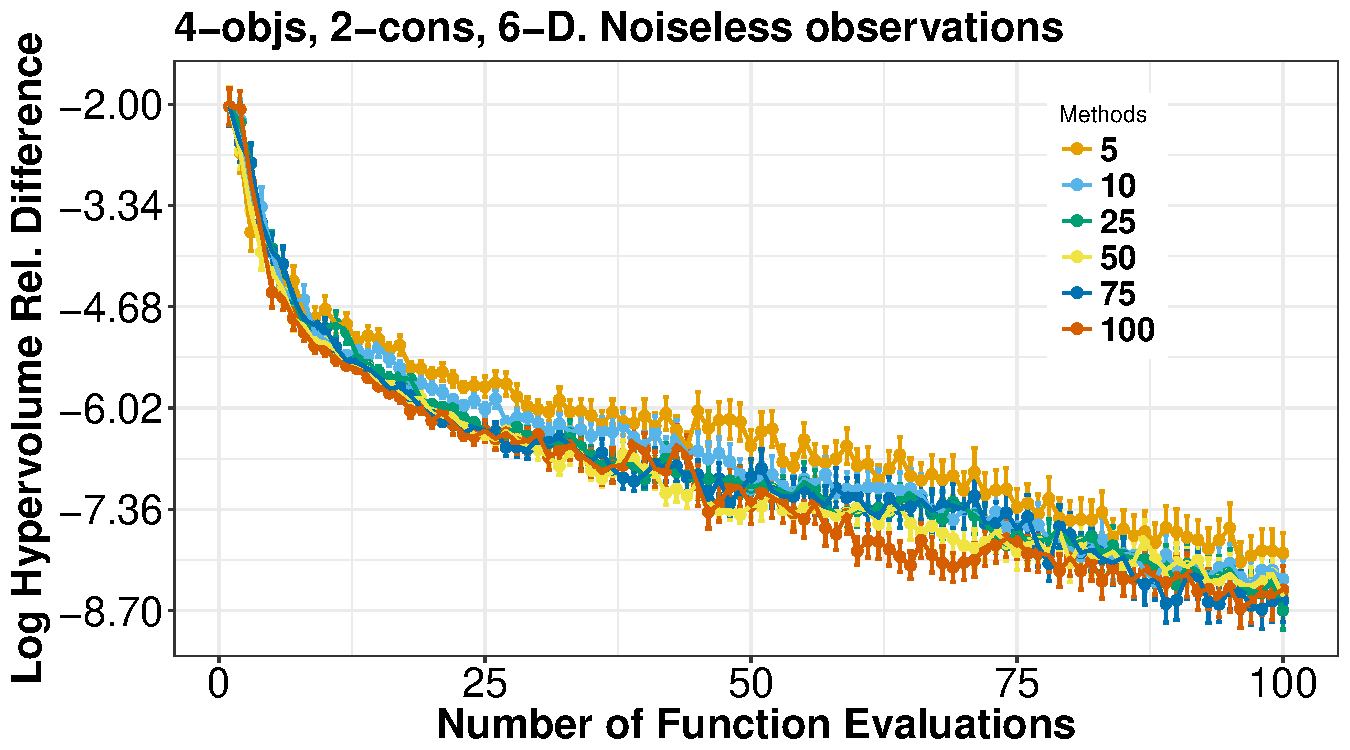
\includegraphics[width=0.75\linewidth]{../Figures/pesmoc/revision/plotParetoSensitivityAnalysis.pdf}
        \caption{Performance of PESMOC in the synthetic experiment for different Pareto set sizes.}
        \end{center}
\label{fig:PPP}
\end{figure*}



\begin{table}[htb]
\centering
\caption{Average time in seconds required to choose
the next evaluation for each size of the Pareto Set sample $\mathcal{X}_{(m)}^\star$. These times do not include the GP fit, in contrast with the average times of the 4 dimensional problem scenario shown in Section 4.2 of the main manuscript.}
{\small
\begin{tabular}{c | c | c}
 \hline
 & \multicolumn{2}{c}{{\bf Time}} \\
 \hline
 {\bf Size of $\mathcal{X}_{(m)} ^\star$} & {\bf Mean} & {\bf Standard Deviation} \\
 \hline
 5 & 95.98& 10.67\\
 10 & 99.05& 11.53\\
 25 & 109.48& 10.92\\
 50 & 133.02& 11.68\\
 75 & 159.90& 15.34\\
 100 & 190.25& 25.71\\
 \hline
\end{tabular}
}
\label{table:times_size}
\end{table}


We observe that by including more points in the Pareto Set, in general, the reuslts of PESMOC improve, as expected.
However, after including around $25$ points the results saturate and no further improvement in performance is observed.
In general one should include as many points as possible in each $\mathcal{X}_{(m)}^\star$. However, including more points in each
sample $\mathcal{X}_{(m) }^\star$ also increases the computational cost, as described in Table \ref{table:times_size}. We observe that choosing $50$
points shows a good trade-off between performance and computational time. In particular, this value gives good results and
is not significantly more expensie than considering $25$ points.

\section{Sensitivity Analysis of the Number of Montecarlo Iterations}

In this section, we present the details of a sensitivity analysis of PESMOC with respect to the number of Montecarlo iterations considered for sampling the hyperparameters of the Gaussian Processes. We have considered the 4-dimensional synthetic problem described in
the main manuscript.  In this problem we have $4$ black-boxes that are sampled from a GP prior. From these, $2$ are objectives
and $2$ are constraints. We performed $100$ experiments in which we evaluate $100$ times the black-boxes and report average
results. We consider a different number of Montecarlo iterations. Namely, 2, 5, 10, 20, 30, 50, 80 and 100. We include a figure
that shows the average relative difference in log scale of the hyper-volume of the recommendation made w.r.t. the hypervolume of the
actual soulution, at each iteration of the optimization process, for each number of Montecarlo iterations.

\begin{figure*}[htb]
        \label{fig:mciters}
        \begin{center}
        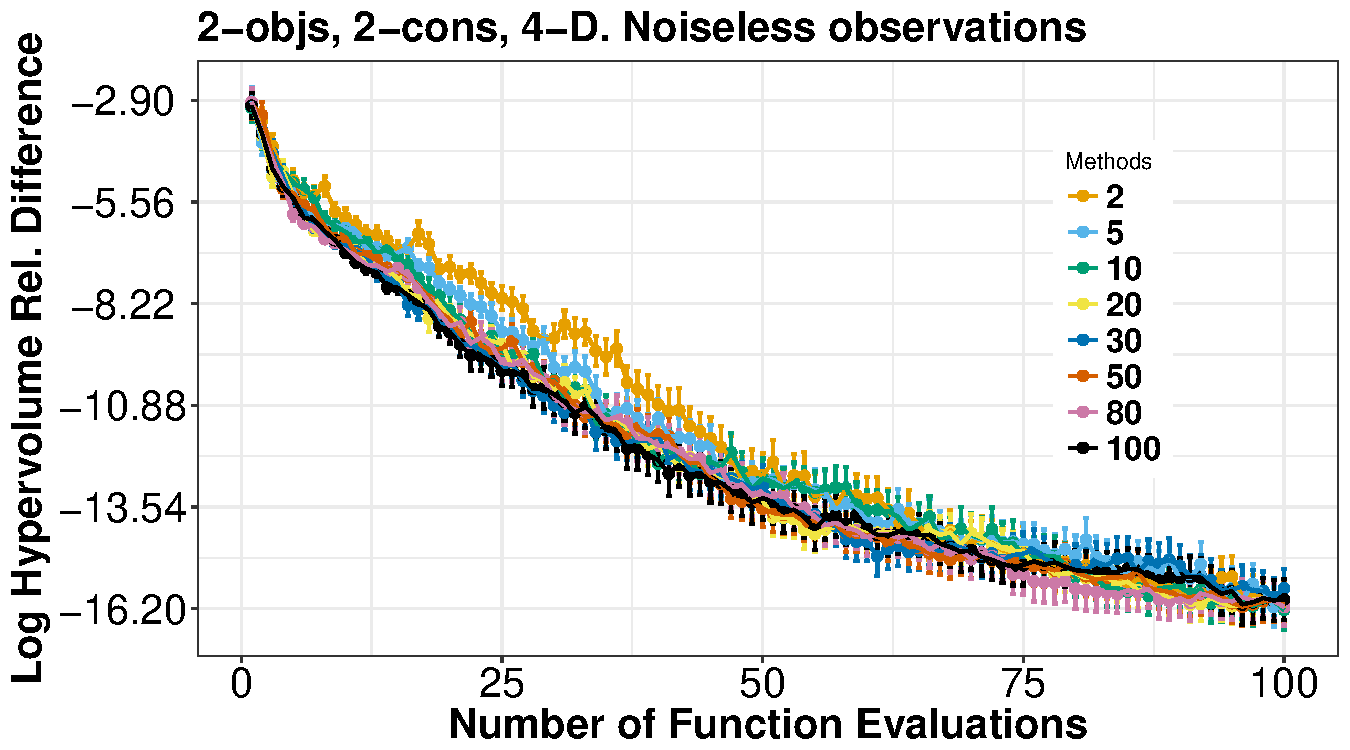
\includegraphics[width=0.75\linewidth]{../Figures/pesmoc/revision/mciters.pdf}
        \caption{Performance of PESMOC in the synthetic experiment for different number of Montecarlo iterations.}
        \end{center}
\end{figure*}

We observe that, for a small number of Montecarlo iterations, in general adding more iterations make the reuslts of PESMOC improve, as expected.
However, after including around $10$ iterations the results saturate and no further improvement in performance is observed.
In general one should include as many number of Montecarlo iterations as possible. However, including more iterations also increases the computational cost, so we observe that choosing $10$ iterations shows a good trade-off between performance and computational time.

\section{Percentage of Infeasible Solutions in Benchmark Experiments}

We show in the next figure the percentage of infeasible solutions for the different benchmark experiments shown in the main manuscript. The plots show the percentage of infeasible solutions for every iteration of Bayesian Optimization on these problems for every tested acquisition function. A higher percentage of infeasible solutions implies that the suggestions provided by the Bayesian Optimization criterion were not located in the feasible region and hence, are poorer that feasible ones. We remind that to be an infeasible point means that the probability of satisfying any of the constraints in that point was lower in at least one of them than 1 minus $\delta$, typically set to $0.05$ in these experiments. This fact may occur, for example for the PESMOC criteria, because the criterion has selected a point that may be close to the border of the feasible region and may be a good point in order to gain information about the Pareto Set, but unfortunately, is infeasible as it lies in the infeasible side of the border, same analogy can be applied for BMOO, which can suggest an infeasible point if it considers it good for optimizing the multiobjective problem. In the random case this does not apply, as the approach performs pure exploration.  At the beggining, the infeasibility percentage of solutions is higher due to he fact that the shape of the constraints is unknown and all the criteria are basically exploring the space, hence, they suggest infeasible solutions with a high probability until the shape of the constraints is reasonably known so the approaches can take the constraints into account for suggesting new points. Then, the infeasibility percentage drops down as iterations are computed.

It is shown that, in average, both PESMOC approaches outperform the other alternatives of multi-objective constrained optimization in infeasibility percentage. The TNK problem has the particular feature that it contains an optimum near one of its constraints, that is the reason why the infeasibility grows around iteration $20$ in all the approaches. This is because as the optimum is more located and the constraint is defined, the methods tend to search in that area, leaving unfeasible results. Once the constraint is defined, they do not search outside of the Feasible Space anymore, and hence, the unfeasible results dissapear. TwoBarTruss problem has the same nature as TNK, with the optimum lying in the frontier of the feasible and infeasible space. We, once again, see how PESMOC decoupled explores massively this area, giving lots of infeasible results in iterations 20 to 30. PESMOC decoupled, as it evaluates every black box separately, learns the shape of these constraints and, as the main manuscript states, it delivers a better solution that the other approaches in less evaluations once it knows the shape of these constraints and it is able to suggest points inside of the feasible space and close to the Pareto set.

\begin{figure*}[htb]
        \begin{tabular}{cc}
                \vspace{-.2cm}
                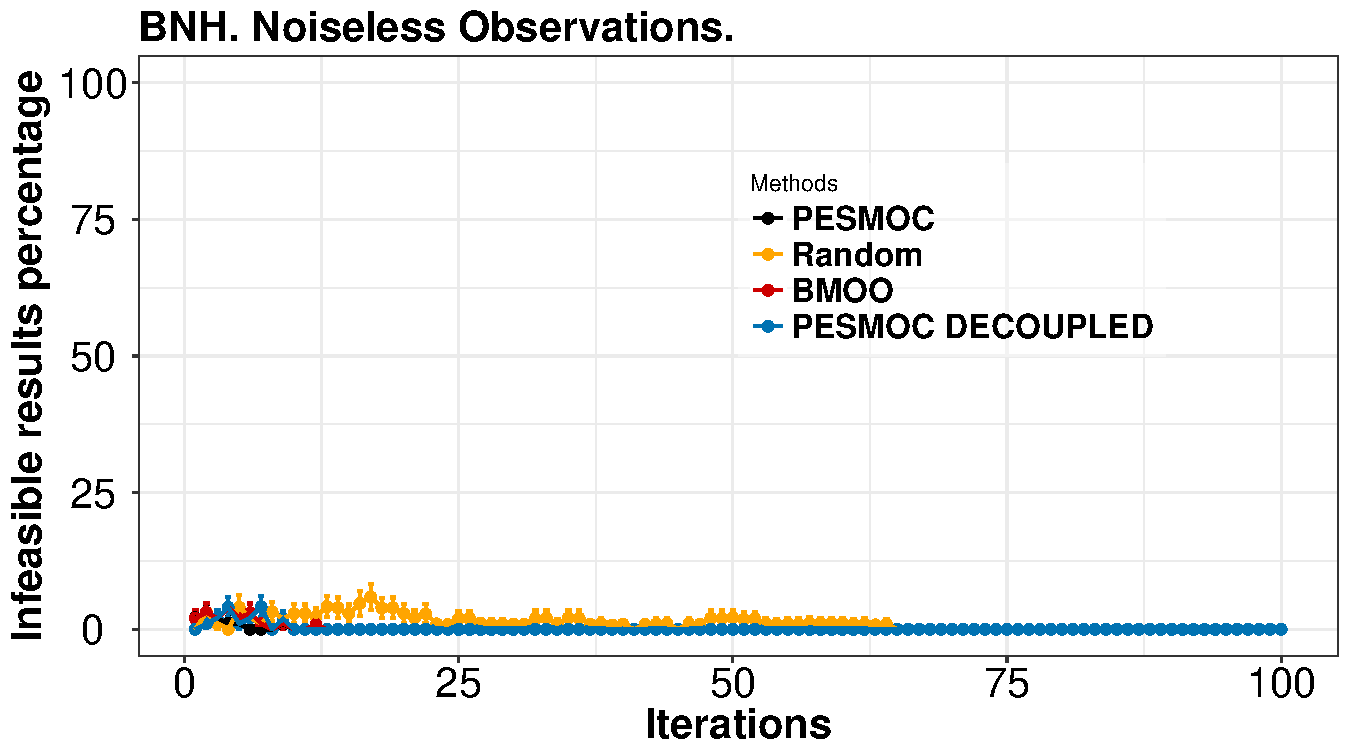
\includegraphics[width=0.475\linewidth]{../Figures/pesmoc/benchmark/BNH_zeros_noiseless} &
                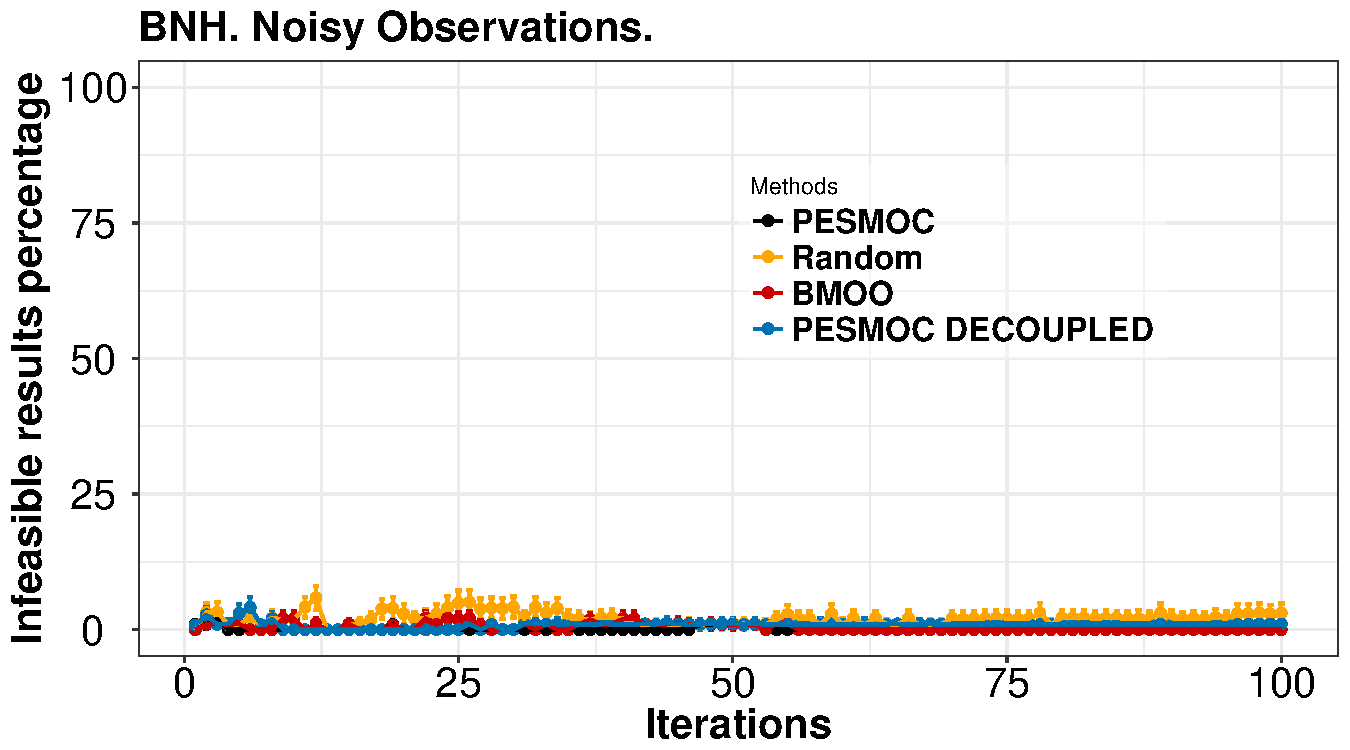
\includegraphics[width=0.475\linewidth]{../Figures/pesmoc/benchmark/BNH_zeros_noisy} \\
                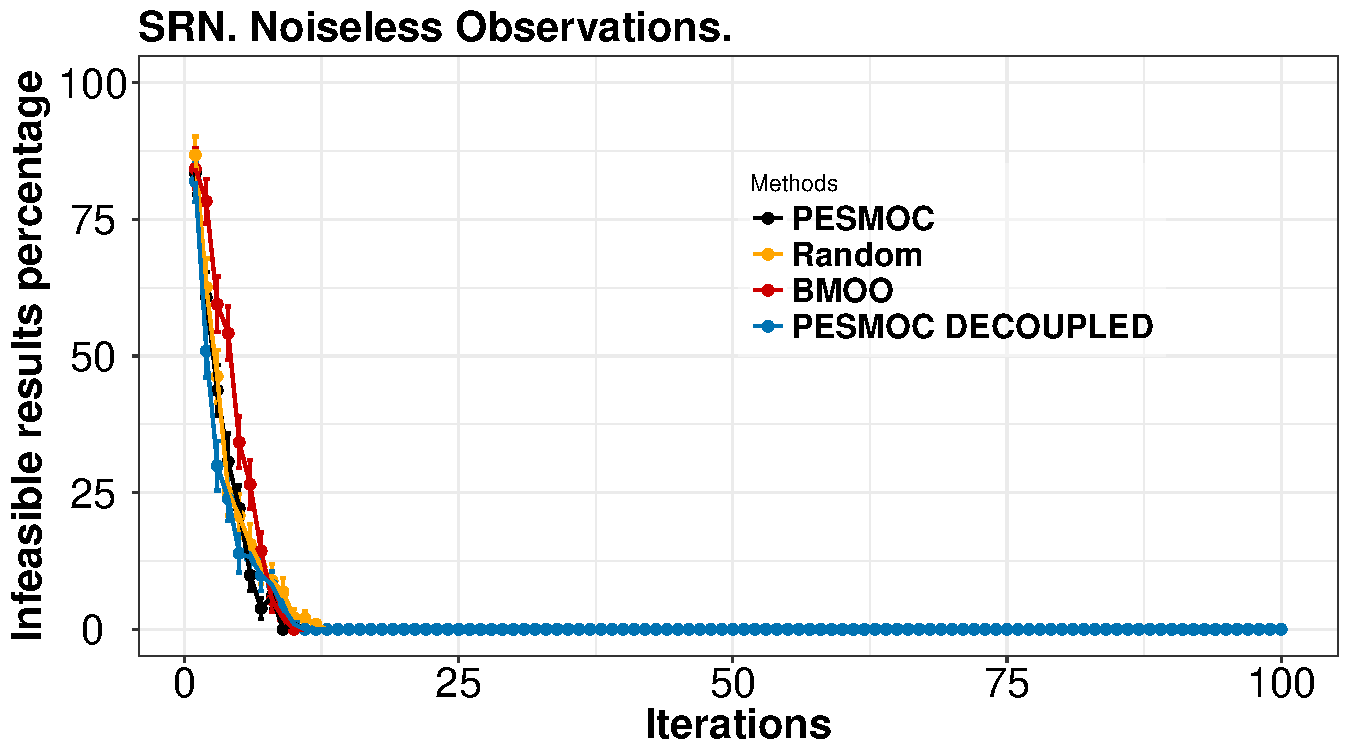
\includegraphics[width=0.475\linewidth]{../Figures/pesmoc/benchmark/SRN_zeros_noiseless} &
                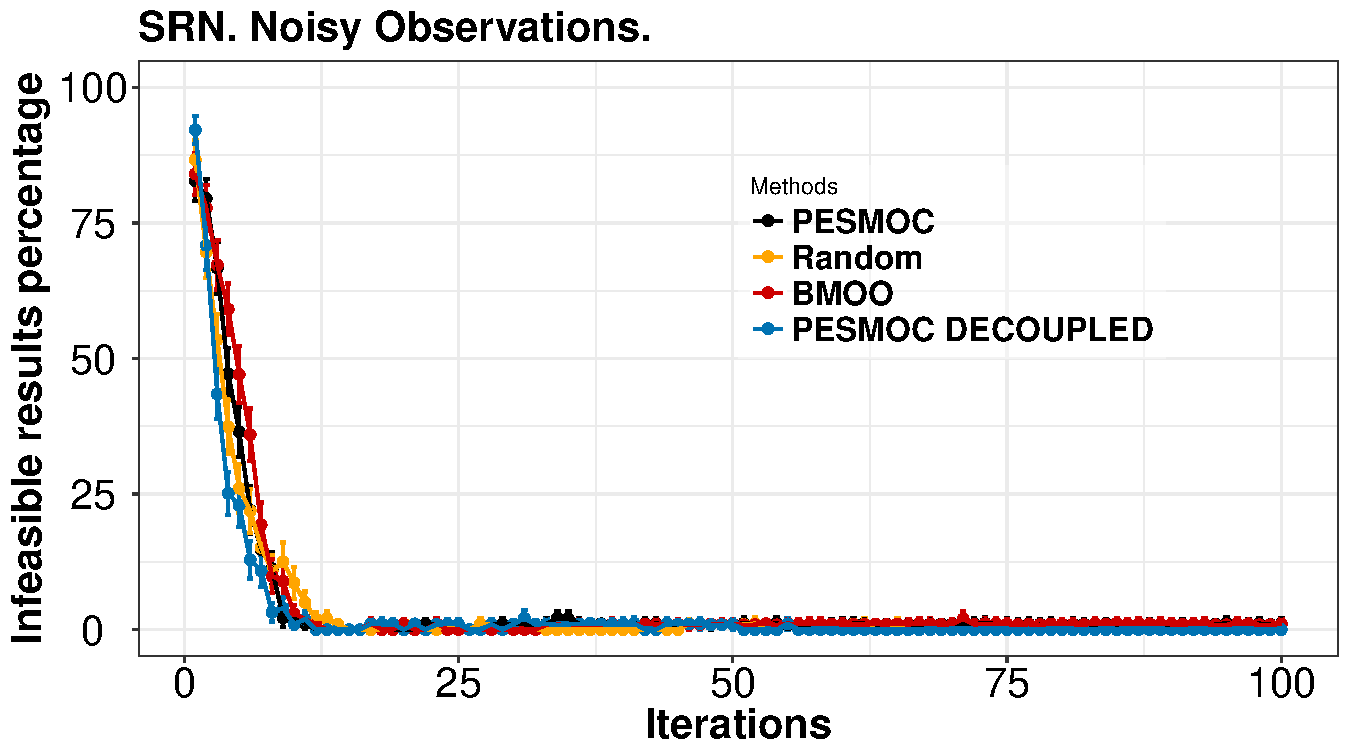
\includegraphics[width=0.475\linewidth]{../Figures/pesmoc/benchmark/SRN_zeros_noisy} \\
                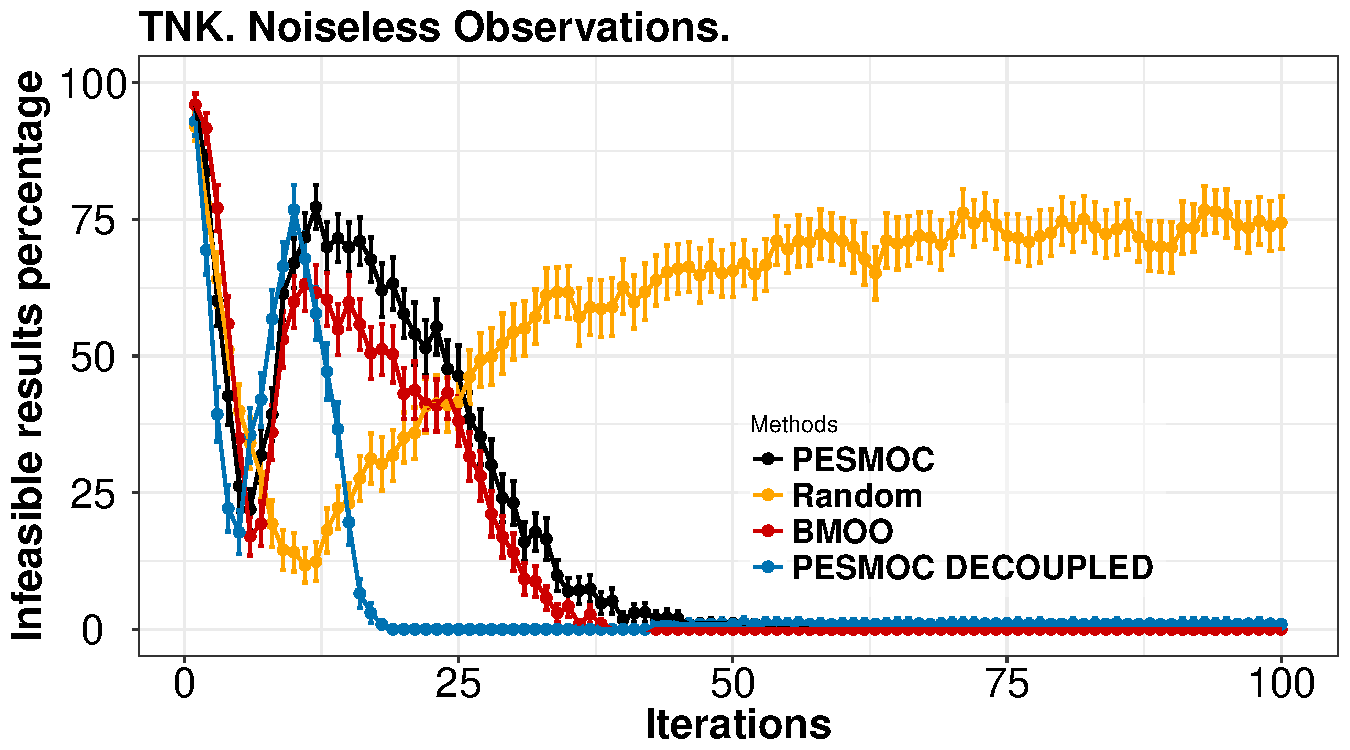
\includegraphics[width=0.475\linewidth]{../Figures/pesmoc/benchmark/TNK_zeros_noiseless} &
                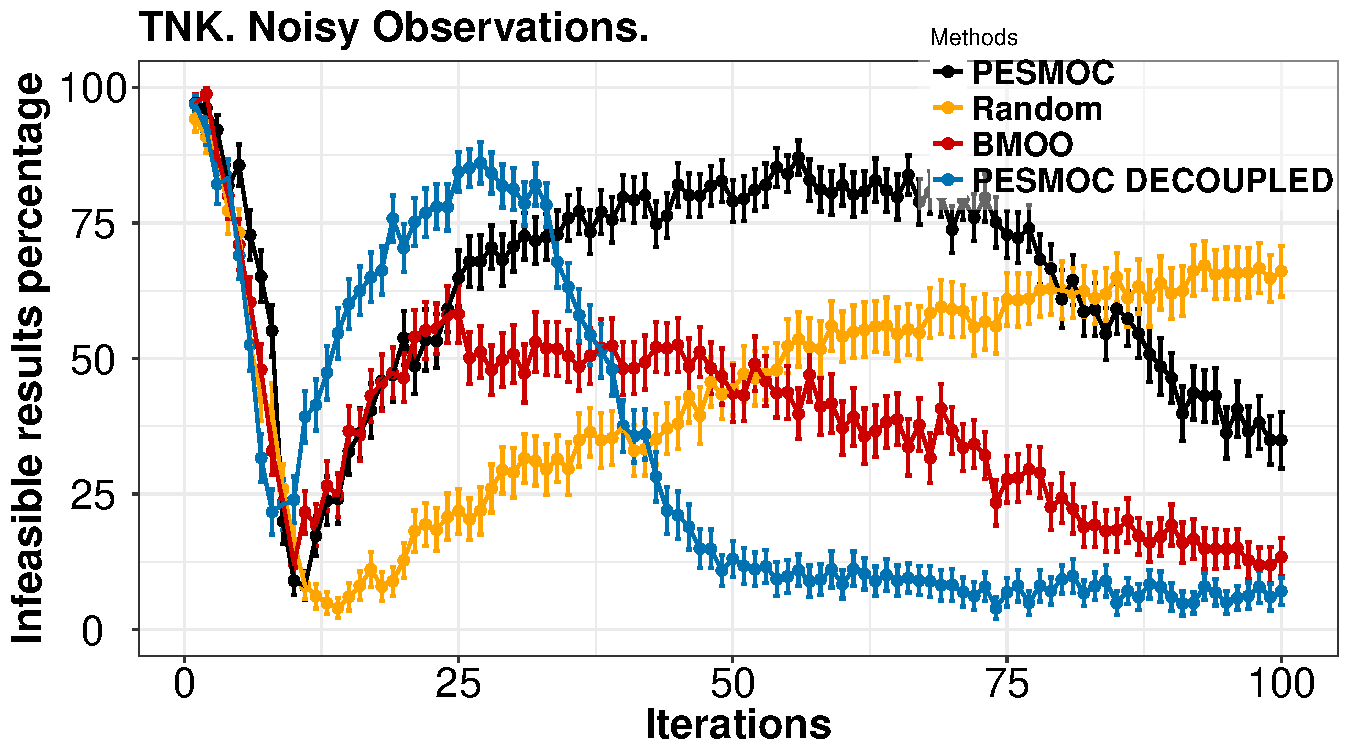
\includegraphics[width=0.475\linewidth]{../Figures/pesmoc/benchmark/TNK_zeros_noisy} \\
                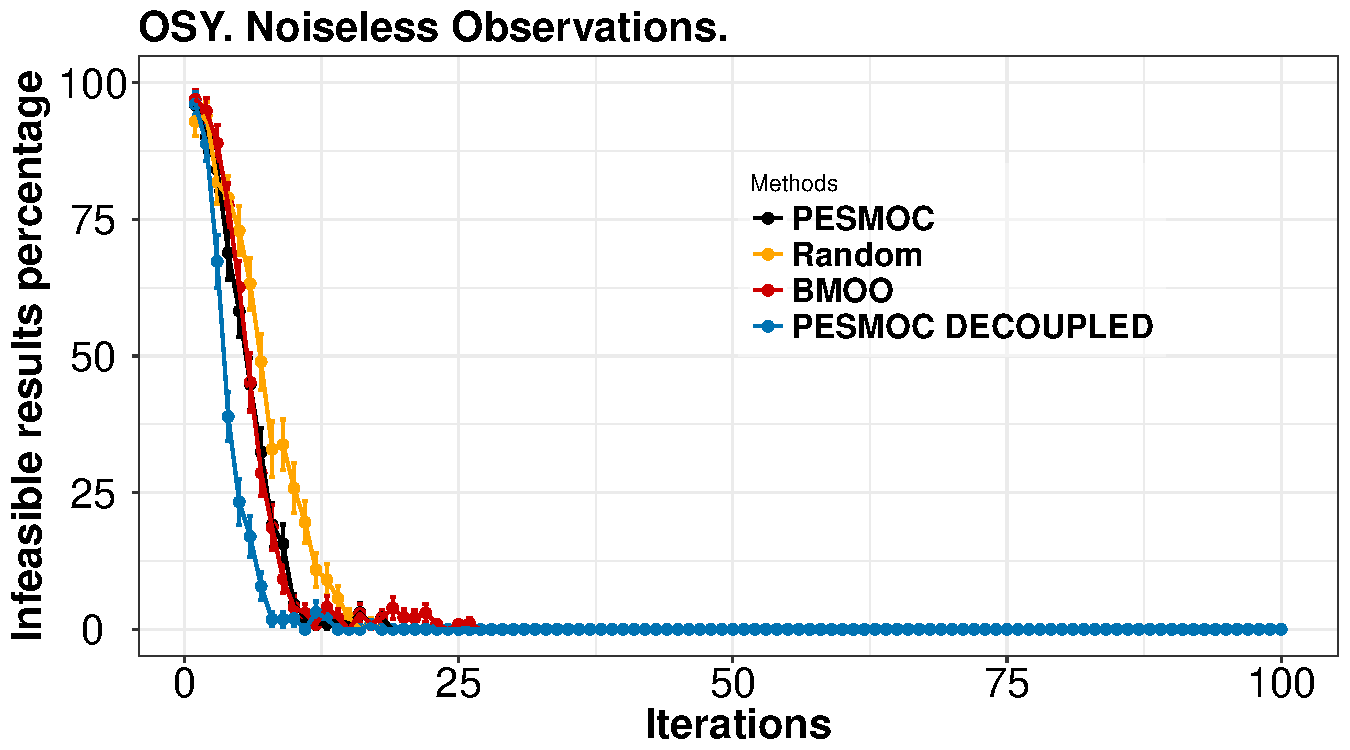
\includegraphics[width=0.475\linewidth]{../Figures/pesmoc/benchmark/OSY_zeros_noiseless} &
                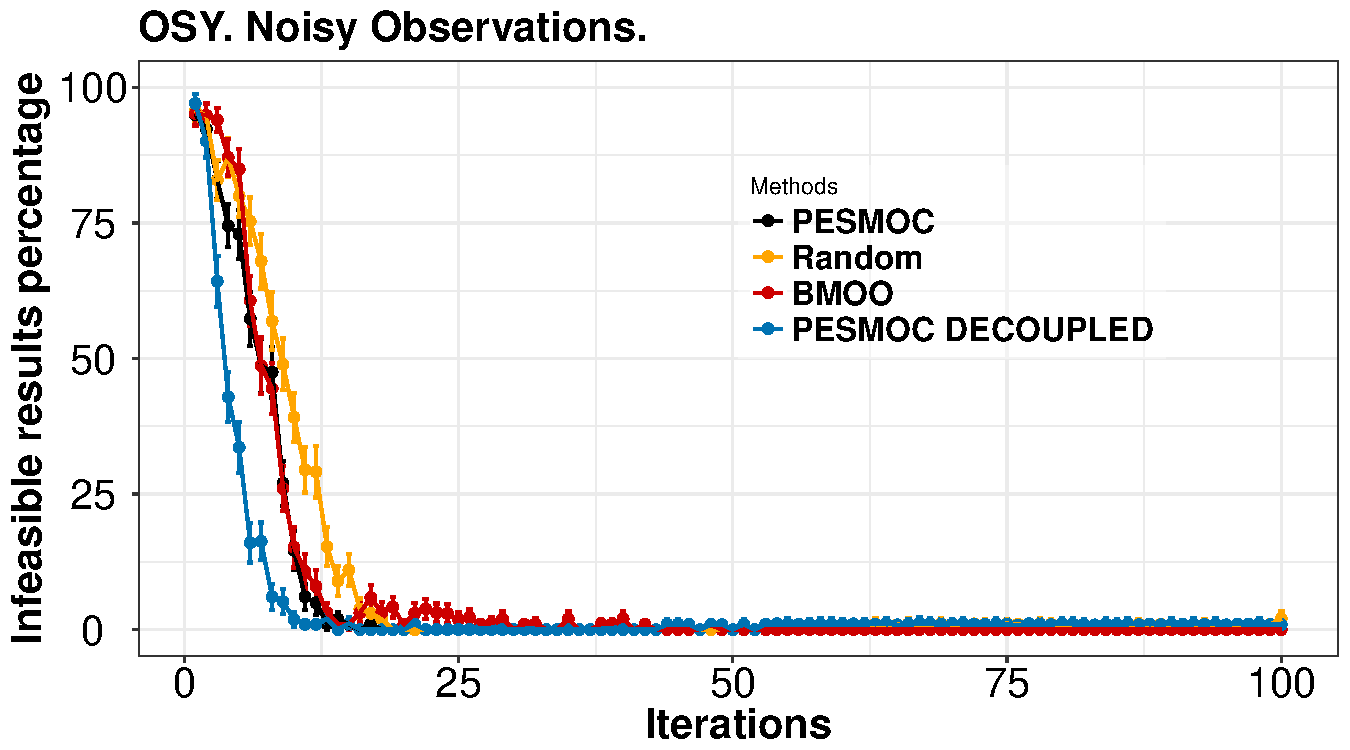
\includegraphics[width=0.475\linewidth]{../Figures/pesmoc/benchmark/OSY_zeros_noisy} \\
        \end{tabular}
        \caption{Percentage of infeasible results in every iteration of experiments BNH, SRN, TNK and OSY.}
        \label{fig:benchmark_results_3}
\end{figure*}

\begin{figure*}[htb]
        \begin{tabular}{cc}
                \vspace{-.2cm}
                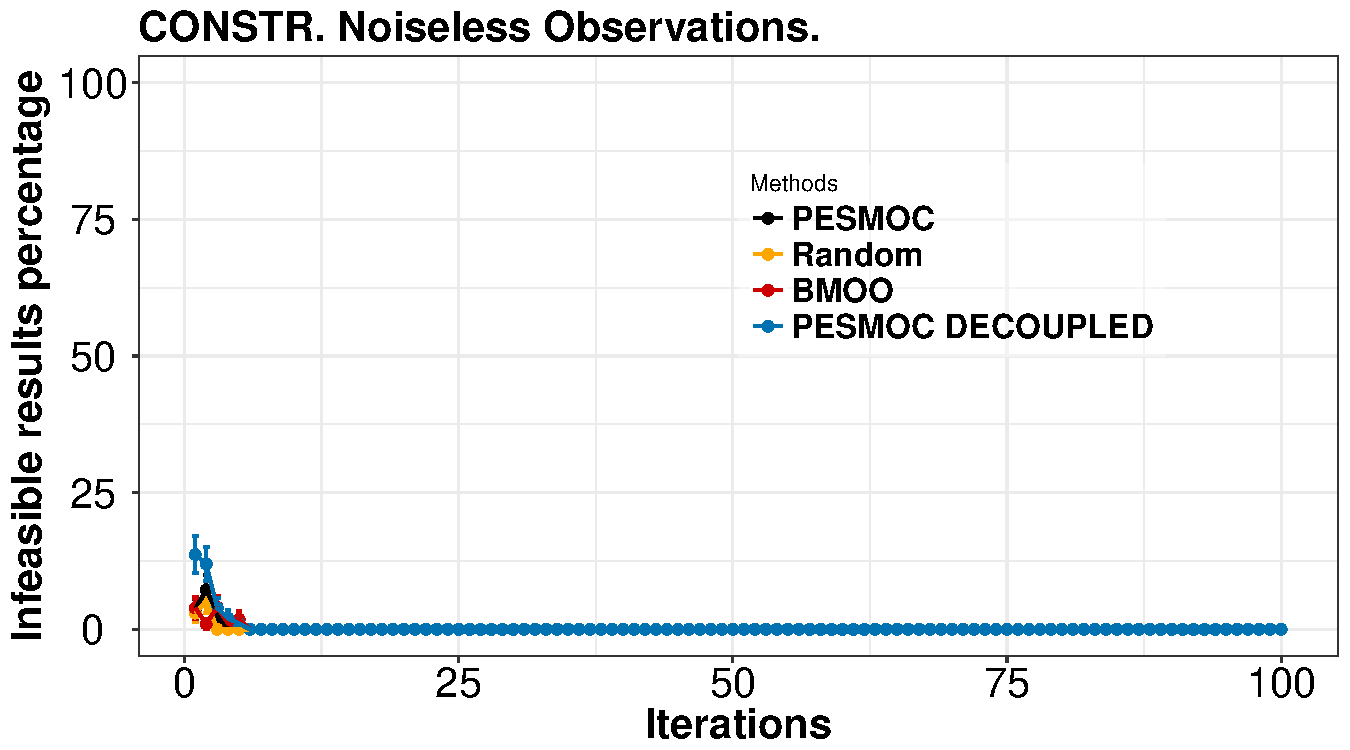
\includegraphics[width=0.475\linewidth]{../Figures/pesmoc/benchmark/CONSTR_zeros_noiseless} &
                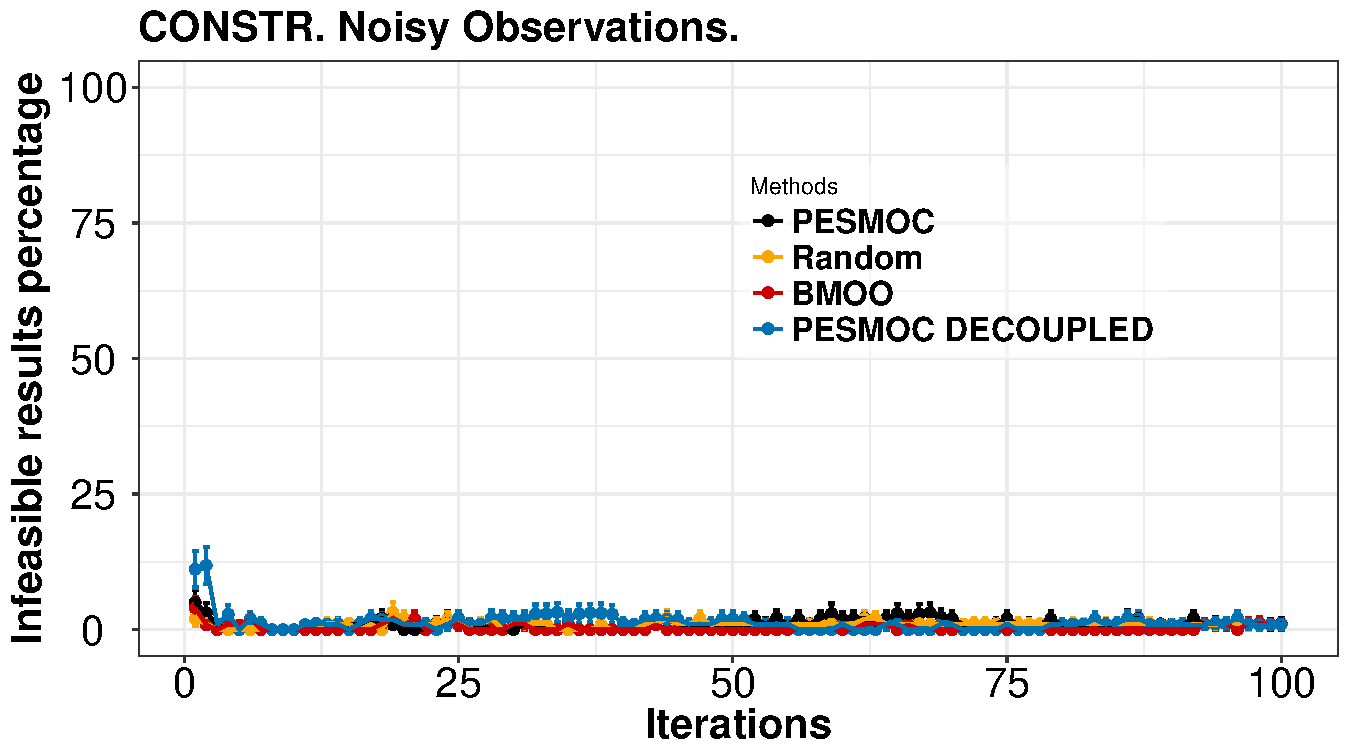
\includegraphics[width=0.475\linewidth]{../Figures/pesmoc/benchmark/CONSTR_zeros_noisy} \\
                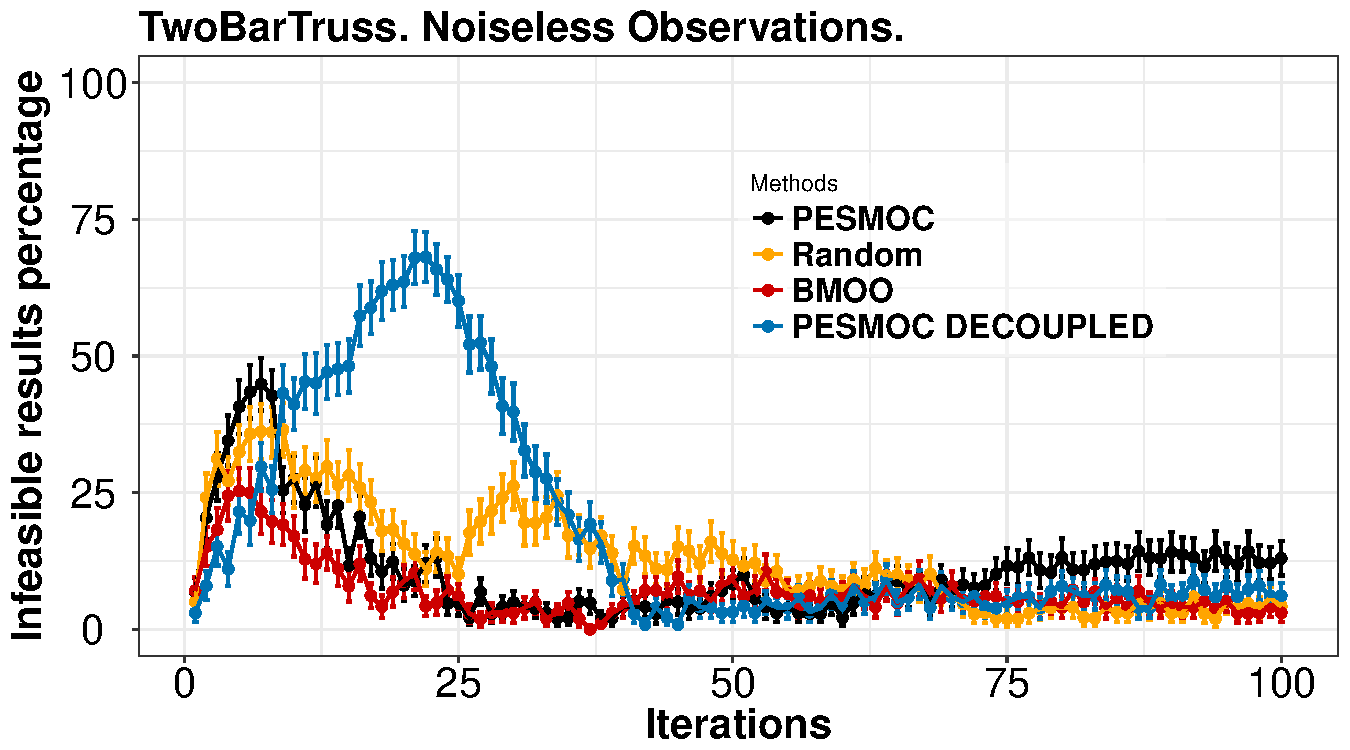
\includegraphics[width=0.475\linewidth]{../Figures/pesmoc/benchmark/TwoBarTruss_zeros_noiseless} &
                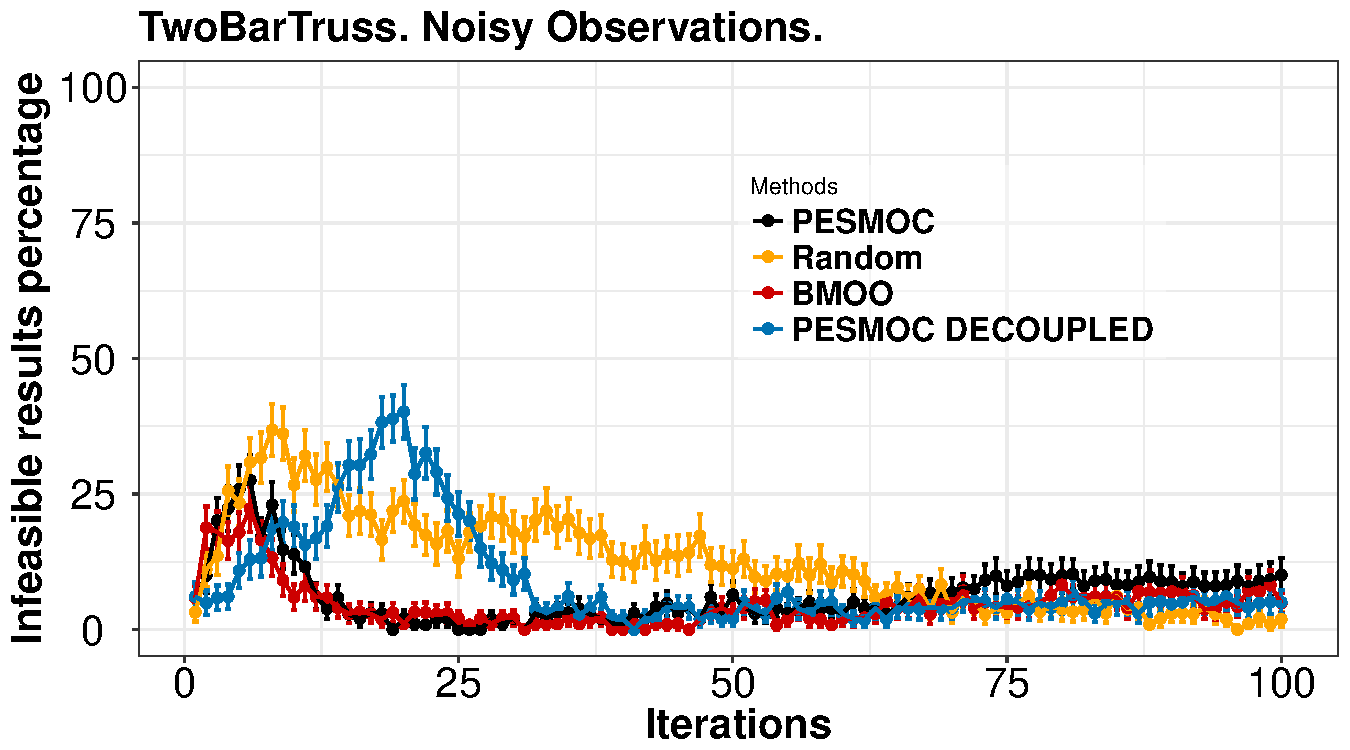
\includegraphics[width=0.475\linewidth]{../Figures/pesmoc/benchmark/TwoBarTruss_zeros_noisy} \\
                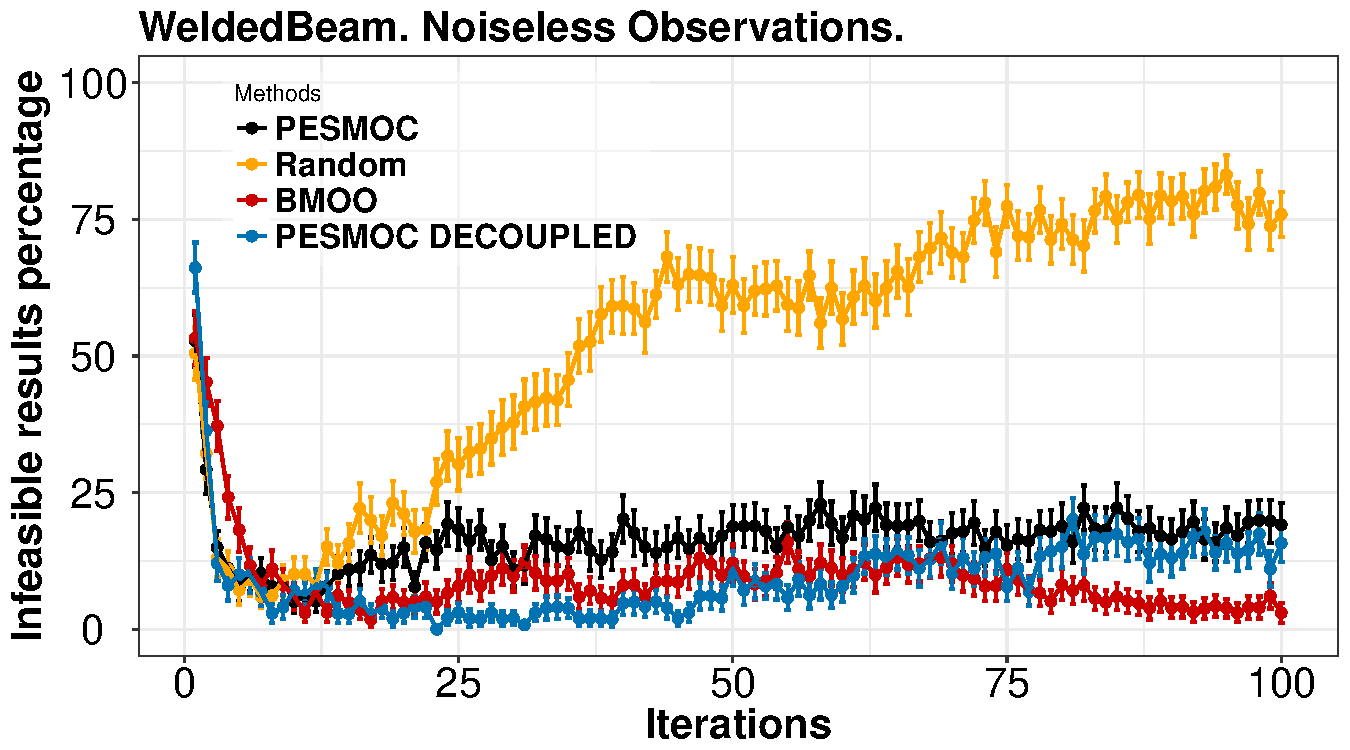
\includegraphics[width=0.475\linewidth]{../Figures/pesmoc/benchmark/WeldedBeam_zeros_noiseless} &
                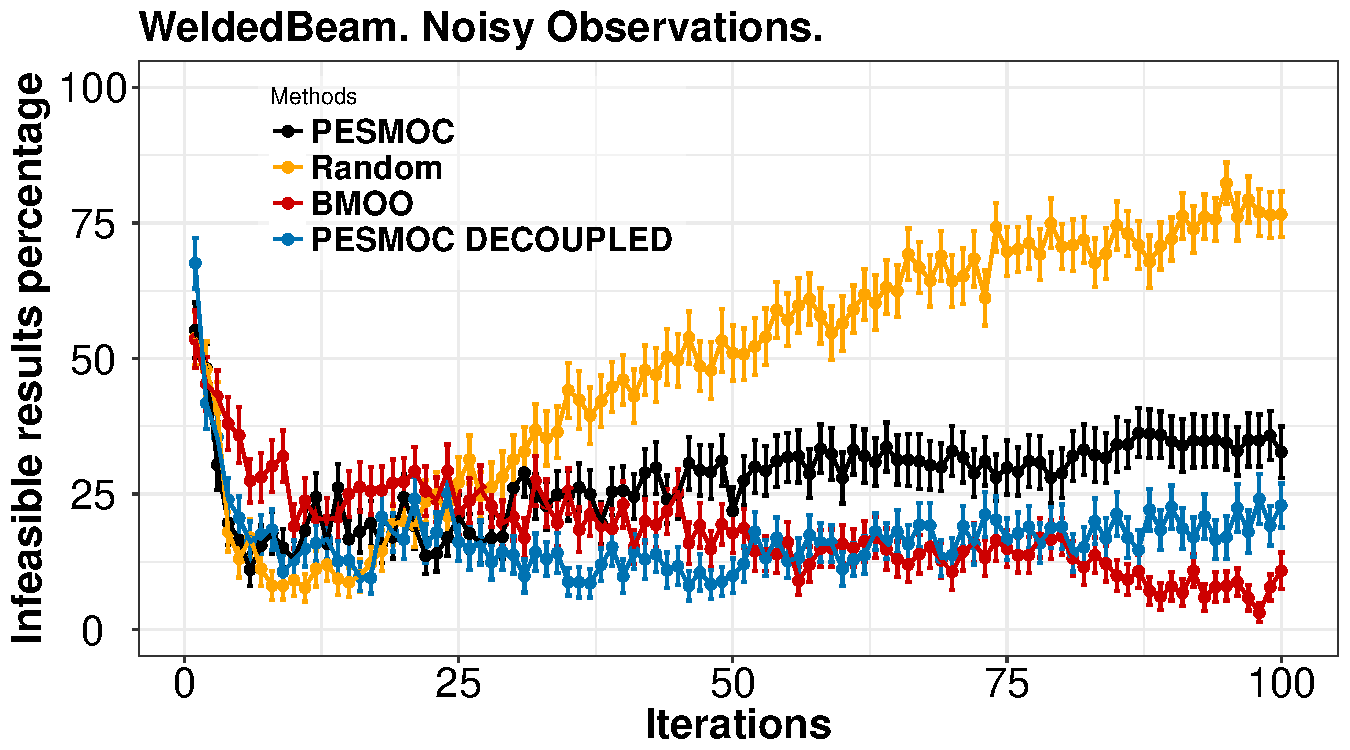
\includegraphics[width=0.475\linewidth]{../Figures/pesmoc/benchmark/WeldedBeam_zeros_noisy} \\
        \end{tabular}
        \caption{Percentage of infeasible results in every iteration of experiments CONSTR, TwoBarTruss and WeldedBeam.}
        \label{fig:benchmark_results_5}
\end{figure*}
